\documentclass[en]{../../../eplsummary}

\usepackage{multirow}
\usepackage{multicol}
\usepackage{graphicx}
\usepackage{listings}

% Footnote in tabular
\usepackage{footnote}
\makesavenoteenv{tabular}
\makesavenoteenv{table}

\hypertitle{Computer Networks : Information transfer}{5}{INGI}{1341}
{Nicolas Houtain\and Benoît Legat\and Gorby Nicolas Ndonda Kabasele\and Florian Thuin}
{Olivier Bonaventure}

\paragraph{French}
There is some part in french because this is a merge between 2 summaries.
It needs to be translated.

\section{Terminology}

\begin{description}
    \item[ADSL] : \textit{Asymmetric Digital Subscriber Lines} le principe est d'avoir un gros lien down pour le particulier et un petit lien en up
    \item[ARP] : \textit{Address Resolution Protocol}
    \item[BPDU] : \textit{Bridge Protocol Data Unit}
    \item[CRC] : \textit{Cyclical Redundancy Check}
    \item[DIFS] : \textit{DCF Interframe Space}. Si une station détecte qu'il n'y a pas eu de transmission WiFi pendant DIFS microsecondes et que l'échange de la dernière trame a réussi, elle a le droit de transmettre. Cette valeur au sein de la gestion des collisions : DIFS = SIFS + (2 * Slot time)
    \item[DNS] : \textit{Domain Name System}. Service permettant de traduire un nom de domaine en informations de plusieurs types qui y sont associées, notamment une IP.
    \item[EIFS] : \textit{Extended Interframe Space}. Similaire au DIFS mais activé uniquement si la dernière frame a échoué. EIFS = Temps de transmission d'un acquittement + SIFS + DIFS.
    \item[HTTP] : \textit{HyperText Transfer Protocol}
    \item[IEEE] : \textit{Institute of Electrical and Electronic Engineers}
    \item[LAN] : \textit{Local Area Network}
    \item[MSL] : \textit{Maximum Segment Life}.
    \item[MTU] : \textit{Maximum Transmission Unit} C'est la taille maximale d'un paquet pouvant être transmis en une seule fois (sans fragmentation) sur une interface.
    \item[Path MTU] : Taille maximale entre une machine source et une machine destination
    \item[PDU] : \textit{Protocole data unit}. Unité de mesure des informations échangées
        dans un réseau informatique.
    \item[RIFS] : \textit{Reduced Interframe Space}.
    \item[SDU] : \textit{Service Data Unit}
    \item[SIFS] : \textit{Short Inter Frame Spacing}. Temps pour une interface sans-fil entre la gestion d'une trame reçue et l'envoi de l'acquittement correspondant (temps pour passer de download à upload pour un routeur).  -> CSMA/CA
    \item[TLV] : \textit{Type Length Value} est un format d'encodage tel que le premier byte est le type, le second la taille totale et puis la valeur.
\end{description}

\section{Layers}

The different layers are represented by the \tabref{layers}.
A router only has the 3 layers: Network, Datalink and Physical. TCP/IP model combine Datalink and Physical layer to Link layer
\begin{table}[!ht]
\centering
	\begin{tabular}{|c|l|c|c|l|}
	\hline
	Layer&Feature&PDU&Id&Protocol \\
	\hline
	\multirow{2}{*}{Application}&&ADU&&BGP,DHCP,DNS,\\&&&&HTTP,FTP\\
	\hline
	\multirow{2}{*}{Transport}&Connectionless unreliable(CRC)&segment&port&UDP,TCP,STCP\\&connection-oriented reliable (graceful) &&&\\
	\hline
	\multirow{2}{*}{Network}&Connectionless unreliable(datagram)&Packet&IP&IPv6,Ipv4,\\&connection-oriented(virtual circuit)&&&OSPF,RIP\\
	\hline
	\multirow{2}{*}{Datalink}&Unreliable (Wifi)use window-based protocol &Frame&MAC&Ethernet,SLIP\\&Reliable(Wires)&&&Wifi,PPP\\
	\hline
	Physical&Unreliable (add/delete/change bit)&bit&&\\
	\hline
	\end{tabular}
\end{table}

\begin{myexem}
  An HTTPS request will use the following protocols in each layer of the OSI model:
  \begin{description}
    \item[Application] HTTP,
    \item[Presentation] SSL,
    \item[Session] TLS,
    \item[Transport] TCP,
    \item[Network] IPv6,
    \item[Datalink] IEEE 802.3 (Ethernet),
    \item[Physical] IEEE 802.3 or IEEE 802.11 (Wireless Local Area Network).
  \end{description}
\end{myexem}

\subsection{Physical Layer}
The Physical Layer service is provided by
\begin{itemize}
  \item \textbf{Electrical cable} twisted pairs or coaxial cables;
  \item \textbf{Optical fiber} multimode or monomode;
  \item \textbf{Wireless} laser for point-to-point and radio-based for spread signal (e.g. WIFI).
\end{itemize}
Its PDU is the bit and the following terms are used
\begin{itemize}
    \item \textbf{Bit rate} : Expressed in bits/sec
    \item \textbf{Bandwith} : Range of frequency usable
\end{itemize}

\subsubsection{Characteristic}

It is \textit{not perfect} (unreliable),
and for us it is like a black box with these characteristics :
\begin{itemize}
    \item \textcolor{red}{change} the value of a bit (\textit{car interference electromagnétique});
    \item deliver \textcolor{red}{more or fewer} bits than requested (\textit{car frequence horloge imprécise})
\end{itemize}

\paragraph{Manchester encoding}
It's an encoding that consist in dividing time in fixed length period. To send a 1, the voltage must be high in the first half of a period and the become low (opposite for zero). It use the symbol InvH (high voltage during last period) and InvB as special marker.

\subsection{Datalink Layer}
The PDU of Datalink Layer service is a \textbf{frame} (\textit{sequence of bit with a particular syntax or structure}) because we want to share data block.
A frame is separated in 3 parts :
\begin{itemize}
    \item \textbf{Header} It contains a flag to tell whether it is an \textcolor{red}{ACK or DATA}, a \textcolor{red}{sequence number} and sometimes the length of the payload.
  \item \textbf{Payload} It contains the information that needs to be transmitted.
  \item \textbf{Error Detection Code} It allows the receiver to detect transmission errors.
    It is either
    \begin{itemize}
        \item a \textsc{hamming code} which is simply a parity bit, it can only detect odd number of errors;
        \item a \textsc{checksum such} as the Internet checksum chosen by the TCP/IP community and the
        Fletcher checksum chosen by the OSI community;
    \item or a \textsc{Cyclic Redundancy Check} (CRC).
        It was slow to implement in software before 1995 and the publication of \cite{feldmeier1995fast}.
        It is now preferred since it has better error detection \cite{stone1998performance}.
        An $n$ bit CRC can detect errors if there are at most $n$
        bits in error or if there is an odd number of bits in error.
    \item an \textsc{hash function} like MD5 or SHA: however, these are built to be collision resistant against
        an active adversary, not random modifications.
        They are also a lot slower than CRC or checksums so they are only used in cryptography.
    \end{itemize}
  \item \textbf{Error Correction Code} It allow the receiver to correct transmission errors.
    No widely used datalink protocol use this.
\end{itemize}

\subsubsection{Framing}

The separation of frames are done using \emph{bit stuffing}
or \emph{character stuffing}.

\begin{description}
    \item[Bit stuffing] : \textbf{01111110} is a frame \textcolor{red}{boundary marker}, so he can't
    be used when we transmit frames.
    \textit{Adds a 0 after 5 consecutive 1 to ensure that this marker is not in the frame}
    \begin{enumerate}
      \item Easy to implement in hardware.
      \item Increase number of bit transmited
    \end{enumerate}
\item[Character stuffing] : In software it's easier to work with character. On rajoute un DLE avant chaque DLE contenu dans les données d'une trame.
    (No imprimable character use as marker)
    Begin of frame : \textsc{DLE STX}, end of frame : \textsc{DLE ETX}.
\end{description}

\paragraph{Note} : Bit stuffing is implemented in hardware and character stuffing is usually
implemented in software.

\subsubsection{Recovering from failures}
We can have errors due to different events:
\begin{enumerate}
  \item The frame has been \textbf{lost} or has been \textbf{corrupted}
    by a transmission error
  \item When we are to slow to treat incoming frames (\textbf{overflow} of the buffer)
\end{enumerate}

\paragraph{ }
Thanks to the ACK flag in the header,
we have 2 types of frames: \textbf{data frame} and \textbf{acknowledgment frame}.
Using to the  \textbf{Error Detection Code}(ex:parity bit), we can try  to recover from failures
of the physical layers and provide a reliable service.

\paragraph{Note: }
Since the \textbf{Physical Layer does not reorder} the bits,
the frames will not be reordered either.
Providing a reliable service it therefore easier than for the Transport Layer that has to cope with the reordering of packets in the Network Layer (it has to discard packets to old packets and have maximal throughput because of that).

\paragraph{Pipelining:  }  This technique  allows  a  sender to  transmit
several  consecutive frames  without being  forced to  wait for  and ack
after each frame.

\subsubsection{Reliable datalink layer}
There are 3 ways of achieving a reliable Datalink Layer.
\begin{enumerate}
  \item \textbf{ABP} :
    The Alternating Bit Protocol is
    a particular case of go-back-n for $n = 2$ (only one bit for the sequence number).
  \item \textbf{Go-back-n} :
    is simple, the receiver discards all out of sequence frames
    and the ACK always contains the last in sequence frame received. It used three variables,
    \textit{lastack,next,maxseq}

    The sender has simply one timer and when it expires, it retransmits \emph{all}
    its unacked frames.

    \begin{center}
    \textit{Good performance if few frame are lost but else the performance is quickly
    drop because of out-sequence frame not accepted and retransmittion of all
unacked frames when it has detected a loss.}
\end{center}

  \item \textbf{Selective Repeat}
      The difference with the go-back-n is that the receiver \textbf{stored out of sequence} frames received, even if cumulative acknowledgement is still used. (\textit{ACK
      contains yet the last in sequence frame received even a out of sequence
  frame is store in buffer})

    The sender has  now a timer  for each frame  of the
    sending window. An ACK covers all the frame in the buffer up to the sequence number acknowledged.

    \begin{itemize}
        \item[$\to$] The ACK sometimes also contains the list of out of sequence frame received (\emph{selective acknowledgement}) to avoid useless retransmission.
    \end{itemize}
\end{enumerate}

\paragraph{Buffer size}
If the sequence number has $n$ bits, we use $2^n$ \textbf{different sequence} numbers.
A \textit{Sliding window} is use to manage the buffer of sequence numbers.

Because the Physical Layer will not reorder the frames,
the maximum window size for the go-back-n is $\bf 2^n-1$ and is $\bf 2^{n-1}$ for the Selective Repeat. 
(Think when all the ack are lost)

\paragraph{  }  Not  all  Datalink Services  provide  a  \emph{reliable}
service. As  a rule  of thumb, datalink  services above  very unreliable
wireless physical services  (e.g. WIFI) does provide  a reliable service
and datalink services above almost reliable wired physical sercies (e.g.
cable or fiber)  do dot include additional  retransmission mechanism and
are also \emph{almost reliable}.

\paragraph{Piggybacking}
When DATA is sent in both directions, an ACK frame and a DATA frame sent by one side are sometimes merged in one because an ACK frame does not need a lot of bit to do its job.
(\textit{Used to reduce the overhead caused by acknowledgements})




\subsection{Building a network}
Network layer is used to send packet between two host that cannot directly relied
by a cable. Host and router \textbf{sending packet}.

There are two possible organisation for the network layer.

\begin{itemize}
    \item \textbf{Data plane :} Protocol and algorithm use to forward data
    \item \textbf{Control plane :} Protocol and algorithm use to make forwarding table
\end{itemize}

\subsubsection{The datagram organisation}

\textit{Inspired by the postal service}, each host is identified by a \textbf{network layer address}.

For each \textsc{packet}, sender must define his address, receiver address and data.

\paragraph{Forwarding}
In datagram organisation, router use \textbf{hop-by-hop} forwarding. (\textit{Each router
forward the packet with his forwarding table})

In a network, \textbf{black-hole} (\textit{when router discard packet because not entry
in his forwarding table for this destination}) and \textbf{cycle} ({packet
consume bandwith}) must be avoiding!


\paragraph{Computing forwarding tables}

\begin{description}
    \item[Port-address table] : Only if we have a \textbf{tree-shapped network} (\textit{drawback}), il suffit d'inspecter les packets reçu pour créer sa table de forwarding sans risquer d'avoir de loop.
        \begin{enumerate}
            \item If the destination address is in the forwarding table, the packet is
                forward on the right interface
            \item Else the packet is send on all interface except the interface
                from wich the packet was receive. It's call \textbf{broadcasting}
                (\textit{drawback})
        \end{enumerate}

        $\to$ The problem with a tree-shapped network is that if a link fails, the network is \textit{split} in two network since there is no redundancy.

        \begin{center}
            \textit{If the network is not a tree, we can also use port-address table but we need to use a distributed algorithm to ensure
            that we have a tree (e.g. Spanning Tree Protocol for Ethernet (Datalink Layer)).}
        \end{center}

    \item[Source routing] : There is no destination address but only the path to reach
        the destination host. Two type of packet :
        \begin{enumerate}
            \item Data packet : to exchange data
            \item Control packet : to discover the path between endhosts. 
                When a router receive a control packet he forwad this one via
                all interface.

                Avoid possible loop because control packet contains a list of \textbf{intermediate nodes}.
        \end{enumerate}
        Complexity is placed on the endhost and network node is simpliest.

\end{description}

\paragraph{Flat or hierachical adresse}
Flat is like number telephone (small match to forwad packet) and hierachical is like a postal adress (smaller forwarding table but adress change when attached to other node\ldots issues with mobile host).

\paragraph{Dealing with heterogeneous datalink}

\begin{enumerate}
    \item \textbf{Retransmitting} : Discard packet and send a control packet to the source to indicate that it cannot forward pacjets longer than 500byte. Source retransmitting the informaiton in smaller packer.
        \begin{center}
            \textit{Router can be really simple and no additionnal operation to perform,
            but may be inefficient because of retransmitting}
        \end{center}
    \item \textbf{Fragmenting} : Router can fragment packet, to way to achieve this :
        \begin{enumerate}
            \item The next router reassembles the fragment
                \begin{center}
                    \textit{Take so much CPU time and memory to fragment 
                    and after reassemble}
                \end{center}
            \item The endhost reassemble the fragment
                \begin{center}
                    \textit{Compromise between the two other}
                \end{center}
        \end{enumerate}
\end{enumerate}

\begin{figure}[h]
    \centering
    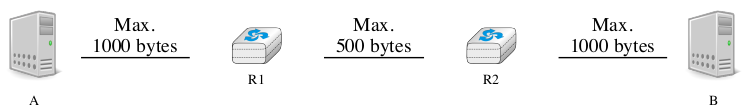
\includegraphics[width=12cm]{heterogeneous.png}
    \caption{Example of heterogeneous datalink layer}
\end{figure}

\subsubsection{Vitual circuit organisation}
Each host has an address. Packet forwarding is not done by looking in the packet destination but by checking 
the label (a int). Enable control over the path used.
\paragraph{label switching} Each node has a label forwarding table. Upon reception of a packet, it forward 
the packet in the direction mappig with the label of the packet. It change the label of the packet. (Lookup in 
O(1)).

\subsubsection{The control plane}
There is two main technique that can be used to maintain the forwarding table in
a network : Distance vector routing and link state routing.

\subsubsection{Distance vector routing}
Allow router discover the destinations reachable inside the network as well as
the shortest path to reach each of these destinations.
(\textit{each link has a associated cost})
\paragraph{Routing table contains} :
\begin{itemize}
    \item $R[d].link$ : outgoing link use to forward paquet to d
    \item $R[d].cost$ : cost of shortest path to d
    \item $R[d].time$ : timestamp of the last distance vector containig destination d
\end{itemize}
When it boots, it send a distance vector with its address at a distance 0.
\paragraph{Routing table update}
Router send regularly its \textbf{distance vector} over all interface.
If a router receiver a distance vector from link l, he only update
the corresponding entry  if either :
\begin{itemize}
    \item $V[d].cost+l.cost < R[d].cost$ : new route smaller thant route already know
    \item[OR]
    \item $R[d].link == l$ : Update of the same route
\end{itemize}
All router send their distance vectore every N seconds. After $3*N$ seconds, the distance vector cost is set to 
$\infty$ if there were no update.
\paragraph{Count to infinity} If two routers send distance vector at the same time, cost keep increasing 
infinitely. Solution $16=\infty$
\paragraph{split horizon} Do not send information to where you have learned it. It is done by making 
specific distance vector for each neighbor.
\subsubsection{Link state routing}
Exchange messages to allow each router to learn the entier network topology, and so
each router is then able to compute its routing table by using a shortest path computation
\footnote{By Dijkstra}

\textbf{Weight} (\textit{Usually symmetric, but it's not a assumption}) of a link can be :
\begin{enumerate}
    \item Unit weight. (\textit{shortest path = lowest intermediate routers})
    \item Proportionnal to the propagation delay
    \item Opposite proportionnal of the bandwith ($\frac{C}{bandwith}$ where C is
    higher than the highest bandwith in the network)
\end{enumerate}
When booting, they send HELLO message to neighboors. HELLO is never fowarded and it is send every N 
seconds. If no HELLO during $k*N$ second, the link considered to have failed.
\paragraph{Static Vs dynamic metric} Experience showed that is was difficult
to tune the dynamic adjustments and ensure that no forwarding loops occur in
the network! \textit{Actualy,} link state routing protocol use metrics
that are manually configured.

\paragraph{Network topology update}
The update is perform by \textbf{link-state packet} that contains :
\begin{itemize}
    \item $LSP.Router$ : identification of the LSP sender
    \item $LSP.age$ : age (\textit{remaining lifetime}) of LSP
    \item $LSP.seq$ : sequence number of LSP
    \item $LSP.Links[]$ : 
\end{itemize}

\paragraph{\textbf{Flooding} algorithm}
Is used to efficiently distribute the LSPs of all router.
To implement this, each router maintains a \textit{link state database} (LSDB) that
contains the most recent LSP for each router. 

$\to$ Router forward a LSP only if he is most recent that the actual LSP on LSDB

\paragraph{\textbf{Reliable flooding}} Router use ack (and retransmissions) to ensure that
all link state packet are successfully transfered to all neighbouring routers. 

When a failure link has been detected, router attached to it send LSP without this link. So all router update 
their LSBD. 
\paragraph{Two-way connectivity} A link is consider failed when one of the router attached to it as detect it.

\subsection{Application}
Two model to organise a networked application. Client-server and peer-to-peer.
To understand each other, the client and the server need to agree on a protocol (format of message + 
organisation of the information flow).
\begin{itemize}
    \item \textbf{Big indian} :  send the most significant byte followed by the least significant byte (the one 
    choose by the Internet)
    \item \textbf{Little indian} : send the least significant byte followed by the most significant byte
\end{itemize}
 In the peer-to-peer model, host act like client and server.


\subsection{The network layer}
Most network use \textbf{datagram organisation} and provide a simple service
which is called the \textcolor{red}{connectionless service}. 

\paragraph{ }Virtuals organisation have a connection systeme based on label.

% Network:
% Datagram: connectionless-> most
% Virtual circuit: connection-> few
%
% Transport
% most on top on datagram so
% UDP: datagraph: connectionless
% TCP: connection oriented
% 
%
\subsection{The transport layer}
This layer improves the service provider by the network to make it useable by application. We only consider
datagram organisation and connectionless service.  IT usually support an unreliable connectionless service.
it need to manage different issue from the network layer :
\begin{multicols}{2}
\begin{itemize}
    \item corrupt data
    \item loose data
    \item not deliver data in-order
    \item upper bound on maximun length of the data
    \item duplicate data
\end{itemize}
\end{multicols}
The main reason for packet loss are the buffer used (discard if buffer full)
The transport layer send \textbf{segment} as PDU
Segment contains \textbf{header} with some control information and
\textbf{payload} from the applicaiton layer.

\begin{center}
    \textit{When a segment is created, this segment is encapsulated by th network layer
    into a packet wich contains the segment as its payload and a network header.
    Packet is then encapsulated in a frame to be transmitted in the datalink layer.}
\end{center}

\paragraph{ }
\textbf{Transport layer} service is, for the most, on top of datagram organisation and so based on connectionless network layer service.

Pour passer du network layer au transport layer, il faut ajouter un méchanisme de
\textbf{gestion des erreurs} et une technique de \textbf{multiplexing} (\textit{via port}).


\subparagraph{ }There is three different service on the transport layer : connectionless service,
connection-oriented service en request-response service.

\subsubsection{Connectionless service}
On envoi les données et le service assure qu'elle arrive.
Utilisé pour le transport de petit SDU.

\begin{description}
    \item[Reliable] : Garantit l'arrivée à coup sur des données. (\textit{difficile à mettre en pratique})
    \item[Unreliable] : Imperfection :
        \begin{itemize}
            \item Garantit seulement une majorité qui arrive (\textit{Souvent ce qui est écarté est du à l'overflow du buffer})
            \item Peut duppliquer les packets sur le réseau
            \item Peut délivrer un SDU différrents
            \item A une taille limité des données
        \end{itemize}
\end{description}
 Ce service apporte deux nouvelles features par rapport au connectionless network layer service: error detection mechanism et multiplexing technique qui permet differencier les  application sur le host.

\subsubsection{Connection-oriented}
Ici il y a trois phases : établir la connection, transferer les SDUs (\textit{la connection est
bidirectionnel}) et fermer la connection.

\begin{itemize}
    \item \textbf{Reliability} : Elle n'est garantie que lorsque la connection est terminé avec un ``gracefully``, sinon des pertes peuvent être observé
\end{itemize}

\paragraph{\textbf{Connection}}

\paragraph{Refus:} Soit de la part du destinataire, soit du provider.
\begin{figure}[h]
    \centering
    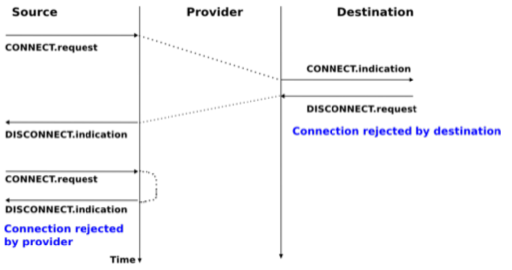
\includegraphics[width=8cm]{refus.png}
    \caption{Refus connection}
\end{figure}

\subparagraph{Three-way handshake:} est utilisé contre l'approche naive de la connexion ``aller-retour''.  Celle ci est définie par l'envoi d'un \textbf{CR}, répondu par \textbf{CA} qui répond \textbf{CA}.

\begin{figure}[h]
    \centering
    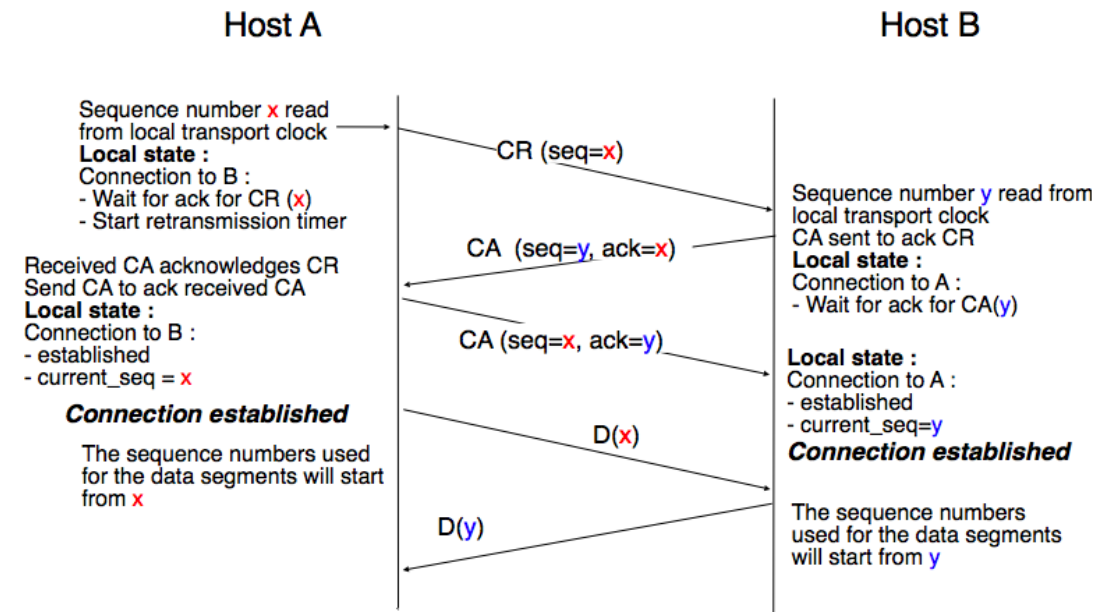
\includegraphics[width=12cm]{threeway.png}
    \caption{Three way handshake connection establishment}
\end{figure}

Pour éviter des \textbf{duplicate transport connection} on utilise un \textbf{transport clock} incremented
every \textit{clock cycle} and after each connection establishment. (\textit{Must continue
to be incremented even if the transport entity stops or reboots})

Implemented with $k$ bits counter and its \textbf{clock cycle} is such that
$2^k \times cycle >> MSL$

\begin{figure}[h]
    \centering
    \begin{tabular}{ccc}
    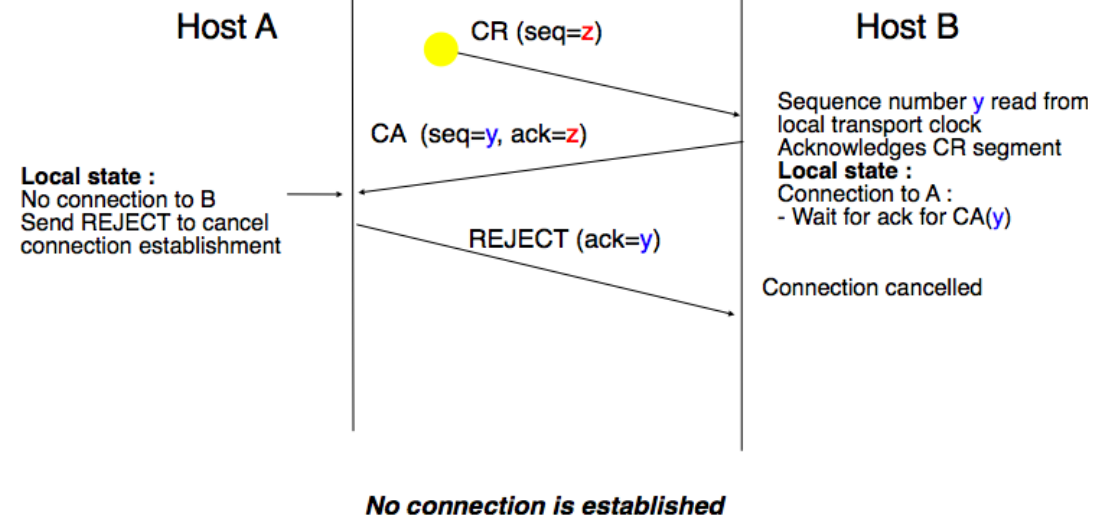
\includegraphics[width=5cm]{three1.png}
    &
    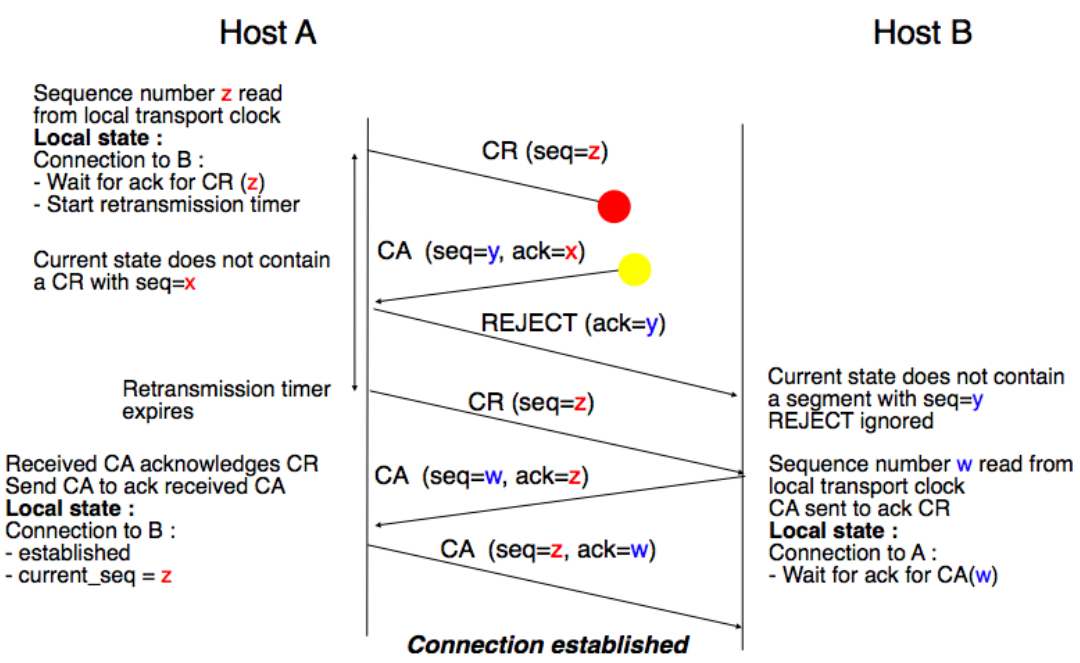
\includegraphics[width=5cm]{three2.png}
    &
    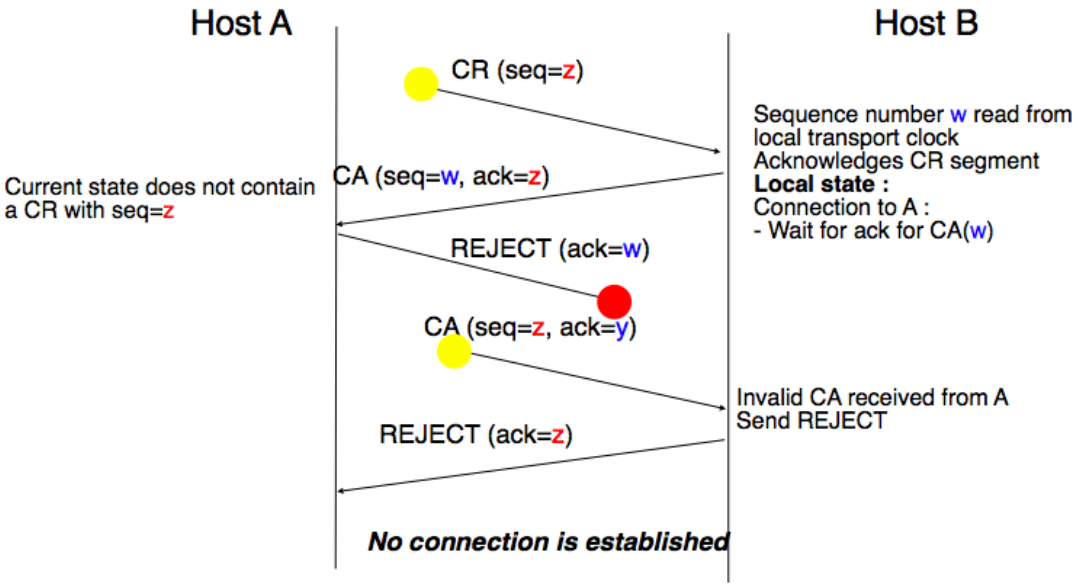
\includegraphics[width=5cm]{three3.png}
    \\
    \multicolumn{3}{c}{$\color{red} \bullet$ when a segment
    is lost and $\color{yellow} \bullet$ when he come from another}
\end{tabular}
\caption{Scenario when transport clock is usefull. }
\end{figure}

\paragraph{\textbf{Data transfert}}
\begin{itemize}
    \item \textsc{message-mode} : On envoie et reçois les messages tels quels. (peu utilisé)
    \item \textsc{stream-mode} : On envoit ici des flux de bytes, et on a besoin de spécifié un délimiter
spécifique pour délimiter les SDU dans le bytestream. (Le provider assure que les bytes arriveront dans le 
même ordre)
\end{itemize}

$\rightarrow$  Le \textbf{Stream-mode}  est utilisé  pour les  reliable
transport protocols,  et le  numéro de séquence  placé dans  la frame
correspond à la position du premier \textbf{byte} du payload dans le bytestream.

\paragraph{Note} : Plusieurs \textbf{différence} par rapport au \textbf{datalink layer}
pour assurer que les données soient délivré.

\begin{enumerate}
    \item Comparé au datalink  layer ou le délai de transmission est fixe
        lorsque deux host  sont connecté, ici le \textbf{delai varie}. (\textit{car les
paquets envoyés  ne prennent pas  forcément le  même path et  il peut
être mis en attente dans le buffer d'un router}).
    \item Les paquets peuvent arriver \textbf{hors séquence} contrairement au datalink layer,Le network peut \textbf{duppliquer} les paquets dans le transport layer
    \item La transmission \textbf{de large SDU}, plus grand que la taille maximal d'un paquet dans le réseau.
\end{enumerate}

\subparagraph{Solution} :
\begin{enumerate}
    \item Pour détecter les erreurs de transmission, comme dans le datalink layer, on utilise un
    CRC ou checksum sur \textbf{chaque} segment.
    \item Pour rendre le protocole reliable, on utilise un numéro de séquence 
        (\textit{correspondant à la position du premier \textbf{byte} du payload dans
        le bytestream}) et des numéro d'ackowledgement. 

        $\to$ 32 ou 64bits nécessaire (pour detecter les délais et parce que les n° s'usent plus vite) plutot que 
        8 dans les datalinks layer protocol.
\end{enumerate}

\paragraph{Go-back-n and selective repeat}
Dans le transport layer on va préférer le \textbf{sélective repeat} puisque cette couche
ne garantit pas l'arrivée en séquence, contrairement au datalink layer.

\paragraph{Buffer variable}
De plus, dans le transport layer, plusieurs application concurrente peuvent communiquer
du coup l'espace mémoire offer à chaque application peut varier ce qui peut rendre la
taille du buffer variable.
Le sender à un \textbf{swin} (\textit{taille de son buffer}), et \textbf{rwin} (\textit{taille du buffer du receiver}). Il considère le minimum des deux comme la window size.

\textbf{Pour éviter un deadlock}, on utilise un persistent timer lorsque le sender reçoit une
window size du receiver égale à 0. Quand le persistent timer expire on force le renvoi du dernier segment.

\paragraph{Excessive timer retransmission} can cause ambiguities if
you make the turn of sliding window\ldots To solve this issues, transport protocol
require the network layer to enforce a \textbf{Maximun Segment Lifetime}.

\textsc{MSL} limits the maximun bandwith of a transport because if it use $n$ bits
for sequence number, then it cannot send mode than $2^n$ segments every MSL.

\paragraph{\textbf{Connection release}}
Soit de manière \textbf{abrute}, soit de manière \textbf{gracefully} càd en fermant
les deux sens de la connections avec un DR suivit d'un ACK.

\subsubsection{Request-response service}
It's a compromise between connectionless service and connection-oriented service. It is used when a host 
need to execute a procedure on another host (\textbf{Remote Call Procedure}). Sending small SDU but 
ensurre the reliable delivery.

\subsection{Naming and addressing}
The network and transport layer rely on adresses that are encoded as fixed size bit
strings. (\textit{for friendly human using}). At first, there was a file (hosts.txt) that mapped name of host to
IP address.
Then, it was decided to organise the name as a tree structure. Each of the top-level domain is managed by 
an organisation that decides how sub-domain names can be registered.
\begin{figure}[h]
    \centering
    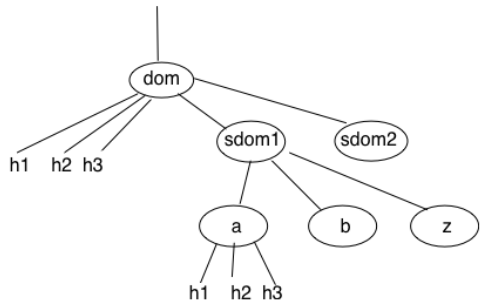
\includegraphics[width=6cm]{internet.png}
    \caption{Internet tree structure}
\end{figure}
This is a key component for the Domain Name Server (distributed database which make the mapping 
between name and IP address ). The nameserver responsible for a domain can answer 2 queries:
\begin{itemize}
	\item The IP address of any host residing inside its domain
	\item Nameserver(s) that are responsible for any direct sub-domain of domain.
\end{itemize}
\paragraph{root nameserver} nameserver that are responsible for ther root of the domain name hierarchy. A 
dozens of them exists and they are synchronized. 
\paragraph{DNS resolver} To avoid client to maintain a list of root server IP, only the resolver keeps them. 
Client contact local DNS resolver if needed.
\subsubsection{Benefit}
Using name instead of address allows:
\begin{itemize}
	\item Keep the same identifier(name) even if the server process move to an other physical layer. No need 
	to inform client about the new server IP address.
	\item If there are many concurrent client on a server, we can add server to reduce load. (Mapping name 
	to a set of address)
\end{itemize}

\subsection{Sharing ressources}
\begin{itemize}
    \item \textbf{Links bandwith} est la ressource la plus importante dans un réseau.
    \item \textbf{buffer} of the network node  est une autre ressource importante.
    \item \textbf{Processing capacity} of node to analyse packet and see on forwarding table.
\end{itemize}

\subsubsection{Organisation to sharing bandwith}
\begin{figure}[h]
    \centering
    \begin{tabular}{ccccc}
    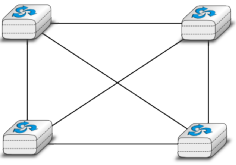
\includegraphics[width=2cm]{fullmesh.png} &
    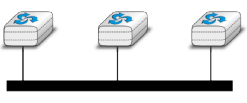
\includegraphics[width=2cm]{bus.png} &
    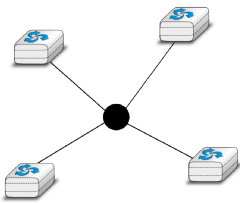
\includegraphics[width=2cm]{star.png} &
    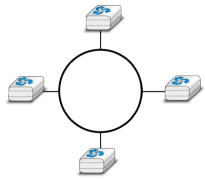
\includegraphics[width=2cm]{circle.png} &
    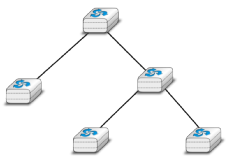
\includegraphics[width=2cm]{tree.png} \\
    Full mesh & Bus & Star & Ring & Tree
\end{tabular}
    \caption{Differents organisations}
\end{figure}

\begin{itemize}
    \item \textbf{A full mesh}
    Le plus efficace, mais nécessite $\frac{n \times (n-1)}{2}$ lien, et chaque
    host doit manager $n-1$ interface ce qui peut vite devenir impossible.

    \item \textbf{Bus organisation}
    Le danger est que si le cable du bus est coupé en deux, le réseau est scindé
    ce qui peut être dur à maintenir.

    \item \textbf{Star organisation}
    Le noeud du centre de l'étoile est vital pour le réseau, mais il permet aussi
    de centraliser le control en un seul point (\textit{C'est un excellent point de
    control et un bon point d'observation}).

    Beaucoup plus facile à maintenir que le bus.

    \item \textbf{Ring organisation}
    Un lien coupe l'entièrete du réseau, c'est pouquoi on utilise souvent un dual-ring.

    \item \textbf{Tree organisation}
    Cela permet de connecter un large nombre de client avec un très petit coût.
\end{itemize}

\subsubsection{Sharing bandwith}

Le partage de bandwith dans les réseaux se veut être \textbf{max-min fairness}(can't allocate more bandwith 
of a flow wihtout reducing the bandwith of an other).

Plusieurs algorithme sont expliqué dans la section Medium Access Control,
on section \ref{medium_access_control}.

\subsubsection{Network congestion}

\textbf{Congestion} when $\sum demand > capacity$.

\paragraph{Congestion collapse}
Cela arrive lorsque le réseau est un peu congestionné, et donc la transmission est ralenti.
Si un protocole tel que \textbf{selective repeat} est utilisé, alors le sender peut
croire que le packet est perdu et donc renvoyé le packet ce qui ne fait qu'augmenter
la congestion!

Pour réguler la congestion, une solution est de connaître la congestion actuel afin que
les hosts ajuste leur bandwith disponible pour diminuer la congestion.

\subparagraph{$\to$} Tant que le buffer est peu ou pas du tout rempli, cela signifie que la demande est plus petite que la capacité et que le buffer sert juste à \textbf{lisser} les demandes dans le temps, sinon il y a une trop de demande pour l'offre de bande passante offerte et on va
arriver à une congestion


\paragraph{Discard mechanism}
On peut choisir d'écarter des paquets qd le buffer est full ou plutot quand il
augmente dangereusement afin de prévenir une congestion!
Toutefois, discard a packet est la solution finale.

\begin{enumerate}
    \item \textbf{Discard the ingoing (tail drop)} : C'est le plus utilisé mais il tend à rester congestionner et
        les applications temps réelles en souffre bcp
    \item \textbf{Discard the next outgoing (drop from front)} : C'est plus judicieux qu'il n'y parait puisque ce paquet
        y est depuis lgtps et on a surement déja détecté la perte (de part la congestion) avant!
    \item \textbf{Random early discard} : Supprime un packet random. (\textit{Permet de supprimer les paquets de différents flow en proportion à leur bandwith}).
\end{enumerate}

\subparagraph{Attention :} supprimer un paquet n'est pas la meilleur solution puisqu'on supprime un paquet qui a consommé des ressources alors qu'on manque justement de ressource!

\paragraph{Forward Explicit Congestion Notification}
Pour les réseaux datagramme,
on utilise un bit pour marquer si le paquet est passé par un endroit congestionné,
et si c'est le cas le receiver envoi un paquet pour informer le sender du degré
de congestion (= $\frac{nbr congestion}{nbr paquet}$)

\paragraph{Backward Explicit Congestion Notification}
Même technique pour les réseaux virtuels, sauf qu'on marque l'acknowledgement.

\paragraph{Control packet}
Allow the network node to send a \textbf{control packet} to the source to indicate
the current congestion level. But their usage is mainly restricted to small network because :
\begin{enumerate}
    \item In large network this packet increase the network load when network is congested
    \item Network node are optimized for forwading packet, not create a packet.
\end{enumerate}

\paragraph{Scheduler mechanism}
Permet d'attribuer une FIFO par flow et un round robin choisit le prochain paquet


\subsubsection{Distributing the load across the network}

\paragraph{Virtual network}
Ici lorsque un host veut envoyer une information, il spécifie la destination et parfois la
bandwith nécessaire. On lui répond si il peut ou non se connecter.. Cette technique
est appellé \textbf{connection admission control}. (\textit{utilisé notament par les téléphones})

\paragraph{Datagram network}
La technique du virtual ne peut être appliqué car dans le datagram un host n'a pas
besoin d'autorisation pour envoyer des packets. See \ref{congestion} pour
certaines techniques de réaction à la congestion.

\paragraph{Shared popular file}
\begin{itemize}
    \item \textbf{Save on multi server} : One server name know by the client and the
        client send a \textsc{query} to know the adress of the server. (\textit{Automatically,
            if there is different server the adresse can change for different people})
    \item \textbf{Using popular bittorent service} : Split the file into different block
        and client needs all block to have file. There is a \textbf{metadata} file that
        contains where each block can be download.
        (\textit{Most deployment of bittorent allow the clients to participate
        to the distribution of blocks})
\end{itemize}

\subsubsection{Medium Access Control (MAC)}
\label{medium_access_control}
The first of the 3 resources that need to be shared inside a network is the link bandwidth 
(\textit{the 2 others are routers processing time and routers buffers}).

\textbf{Collisions} happens when two hosts try to send a frame simultaneously.
It is the principal source of errors in Local Area Network.

\paragraph{ }
There are 2 types of MAC : 
\begin{itemize}
    \item \textbf{Deterministic} or pessimistic MACs: They ensure that there will be \emph{no} collision.
    They are more appropriate in network where the load is constant (e.g. telephone, radio).
\item \textbf{Stochastics} or optimistic MACS: They try to minimize the number of collisions.
    They are more appropriate in network where the load has an on-off behaviour (e.g. internet).
\end{itemize}

\paragraph{\textbf{Deterministic MAC}}
The deterministic MACs are the following (the 3 first are \emph{static} allocation methods)
\begin{itemize}
    \item[-] \textbf{Frequency Division Multiplexing} :
    If wireless medium, we can give a different frequency for devices.
  \item[-] \textbf{Wavelength Division Multiplexing} :
    In optical medium, we can give a different wavelength for devices.
  \item[-] \textbf{Time Division Multiplexing} :
    In any medium, we can just divide the time in separate slots and assign the slots to devices
    statically or dynamically.
  \item[-] \textbf{IEEE 802.4 (Token Bus Network)} :
    Transmit a token in a network of bus topology.
    To transmit data, wait for the token and then transmit the data instead of the token.
    Once the data transmitted, put the token back in the network.
  \item[-] \textbf{IEEE 802.5 (Token Ring Network)} :
    Same than 802.4 but with a ring topology. 

	\item[-] \textbf{Deterministic Medium Acces Control (DMAC) } : Example with the Token Ring 
	\begin{itemize}
		\item Node have two mode: listen mode where they forward the  signal they receive inserting a one bit delay. Andtransmit mode where they have the token and they  transmit data. 
		\item There is a special node called \textbf{Monitor} which ensure that the token always travel on the token ring (it insert a token size delay). 
		\item Node stop transmitting when it get its own bit. Beginning of the token is the beginning of the data frame so node can know with a bit if it's a token or a data.
		\item A station can't retain the token for more than Token Holding Time.
    \end{itemize}
\end{itemize}

\paragraph{\textbf{Stochastics MAC}}

\begin{itemize}
    \item[-] \textbf{[slotted] ALOHA} : First approach is ALOHA.
        When no ack is received, we wait a \textcolor{red}{random time} instead of a fixed time to \textbf{avoid synchronisation} with other hosts.

A simple improvement is \textbf{slotted} ALOHA which divides the times into slots of the same size than the time require to transmit one frame.
Transmisssion are only allowed to start at the beginning of a time slot.
This avoids collison on part of a frame since that require the frame to be completely retransmitted anyway.

\item[-] \textbf{[non-]persistent Carrier Sense Multiple Access (CSMA)} :
An improvement to ALOHA is \textbf{persistent} CSMA which sense the network before sending a frame but does not wait random time.

To avoid synchronisation on with CSMA, \textbf{non-persistent} CSMA waits a random time before sensing the network, it is is not free, it will wait a random time before sensing it again.

\item [More] improvements can be made but depends on the technology

\item[-] \textbf{CSMA/CD for IEEE 802.3 (Ethernet)} :
On ethernet, a host is able to detect a collision while it is listening.

If $\tau$ is the diameter of the network (the largest time between 2 host),
we know that if a frame of length $2\tau$ has a collision, the sending host \textbf{will sense it} (as any 
other hosts by the way).
We therefore enforce $2\tau$ as the minimum frame size.

$\to$ Since Ethernet has not many transmission errors, CSMA/CD does \textbf{not uses acknowledgment} to 
avoid the collisions they would cause. Also because the sender knows when there are a collision, it knows 
when a transmission error occurs.

The time waited by the hosts when a collision is detected is random to avoid synchronisation,
is a multiple of $2\tau$ for the same reason as slotted ALOHA and is selected in a range multiplied by 2 after each collision,
this is called a \emph{binary exponential back-off}.

\item[-] \textbf{CSMA/CA for IEEE 802.11 (WiFi)}

\begin{description}
    \item[SIFS] : This is required to \textbf{switch} between upload and download in a router.
    \item[DIFS] : The channel must be idle DIFS (time) before a device can transmit \textbf{after the previous frame was received correctly}.
    \item[EIFS] : the time the device must sense the channel idle \textbf{after the previous frame was corrupted} before transmitting.
    \item $$SIFS < DIFS < EIFS$$
\end{description}

There is a \textbf{random} exponentonialy \textit{backoff timer} in addition of \textsc{DIFS} or \textsc{EIFS}
before sending a frame. (\textit{This timer is frozen when the channel is busy!})

Another problem with wireless is \textit{hidden station problem}, where you don't reveive 
the signal of other device (and so when the channel is busy).

To solve this, there is two control frame \textsc{RTS} (ask for a delay reservation)
and \textsc{CTS} (to comfirm reservation). (\textit{small size to minimize collision}).
All host are informed of the reservation.

\begin{figure}[h]
    \centering
    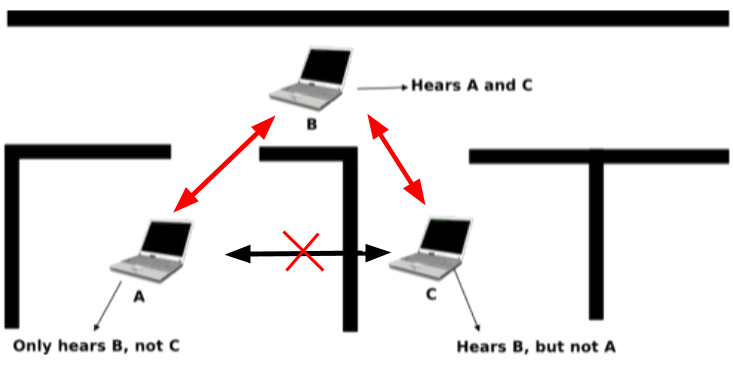
\includegraphics[width=6cm]{hiddenstation.png}
    \caption{Hidden station problem}
\end{figure}

\end{itemize}


\subsubsection{Congestion control}
\label{congestion}

Pour supprimer la \textbf{congestion collapse}, les hosts doivent réguler leur taux
de transmission. (\textit{Note qu'il y a d'autre méchanisme pour réguler tel que celui
basé sur les crédits})

\paragraph{Goals of congestion control} for a set of i hosts :
\begin{itemize}
    \item Doit supprimer la congestion càd $\forall_t \sum r_i(t) \leq R$
    \item Efficace càd $\forall_t \sum r_i(t) \approx R$
    \item Juste pour tous ($\to$ max-min fairness est l'utopie)
\end{itemize}

Such a mechanism can be implemented in \textit{transport layer} or in the \textit{network
layer}. (TCP/IP implements this in transport)

\paragraph{Control de congestion} est un algorithme qui adapte le taux de congestion :
\begin{enumerate}
    \item \textbf{Multiplicative decreasing} si il y congestion : $rate =  rate*\beta, \quad \beta <1$
    \item \textbf{Additive increasing} sinon :  $rate =  rate + \alpha, \quad \alpha>0$
\end{enumerate}

\paragraph{Congestion control in window-based transport protocol}
Reduce the window size can reduce the congestion because a device cannot
send data faster than : $$\frac{Window}{rtt}, \textrm{ where window is current sending window} $$

\subparagraph{Limit window size}
\begin{itemize}
    \item[-] Rappel : \textit{swin} is the size of sending window, \textit{rwin} size
        of receiving window and now \textit{cwin} is the congestion window.
    \item[-] \textbf{Congestion window} : limits the sending window. 

        \textit{swin} = $min( swin, cwin )$
\end{itemize}

When start, \textit{cwin} is set to one segment and it increases (\textit{additive}) by one every RRT when there is no congestion , else it is divided by two (\textit{multiplicative}).

\paragraph{Note: }
\begin{description}
    \item Congestion is detected when a packet is loss.
    \item Mild congestion : 3 duplicate ack ($\to$ Fast retransmit)
    \item Severe congestion : restransmittion timer expire
        \end{description}

\subsection{The reference models}


\begin{table}[h]
    \begin{tabular}{|c|c|c|c|}
        \hline
        Application & SDU     &                                        &  \\
        \hline
        Transport   & Segment & Connectionless unreliable              & connect to network  \\
                    &         & connection-oriented often reliable   & \\
        \hline
        Network     & Packet  & Unreliable                             & connect to network \\
        \hline
        Datalink    & Frame   & Reliable (if use ack and error detect) & directly connect to device \\
        \hline
        Physical    & Bit     & Unreliable                             & directly connect to device \\
        \hline
    \end{tabular}
    \caption{Reference models}
\end{table}

\paragraph{TCP/IP reference model} The same but physical layer and datalink layer are combined in link layer.
\paragraph{Model OSI} There are a session and a presentation layer before the application layer. Session layer deals with the organisation and the synchronization of the message/data exchanged with presentation entity. Presentation layer deals with how to represents the information. 

\section{Protocols}

\subsection{Application layer}
A application use connection less service or connection-oriented service
and are \textcolor{red}{identified} by a port number and a network adress (\textit{IPv4 or IPv6}). TCP is also called the byte-stream mode service and UDP the datagram service.

\begin{description}
    \item IPv4 : 32 bits wide
    \item IPv4 : 128 bits wide
\end{description}

\subsection{DNS}

\begin{figure}[h]
    \centering
    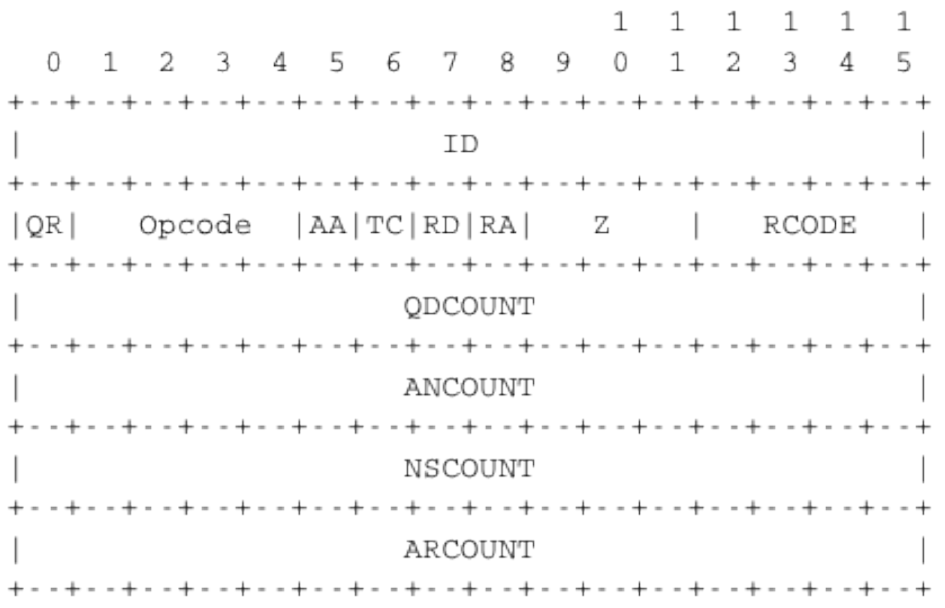
\includegraphics[width=10cm]{dnsheader.png}
    \caption{DNS header}
\end{figure}
DNS runs usually above datagram service. The message is divided in five part, the 3 first one are mandatory, the other 2 last one are optional. In the DNS message header, there is an identifier to match request to answer an inforrmation on authority server (who manage). A request is recursive when resolver recurse through DNS hierarchy to retrieve answer. 
\paragraph{Resource Record} 
\begin{itemize}
	\item[Time-to-Live] How long the client can keep the Resource Record inside is cache.
	\item[Type] Field in the record to specify if IPv4(A) or IPv6(AAAA)
\end{itemize}

DNS permet d'obtenir l'adresse qui correpond à un certain nom, mais on peut
faire un reverser DNS pour obtenir le nom d'une adresse.

\subsection{Electronic mail}

A \textbf{email system} is composed :
\begin{itemize}
    \item A message format
    \item Protocols : to exchange between host and server
    \item Client software : to create/read mail
    \item Software : to efficiently exchange email by server
\end{itemize}
 
\begin{figure}[h]
    \centering
    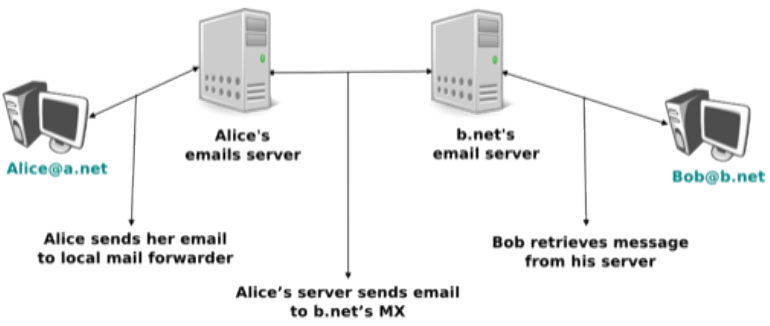
\includegraphics[width=10cm]{mail.png}
    \caption{Simplified architecture mail}
\end{figure}

\subsubsection{Email message}
Email message are composed of two part : a \textbf{header} (\textit{From*, Date*, To*, Subject,  cc, bcc}) and a \textbf{body}. (* are mandatory)

Line to separate header and body is empty and contains only CR and LF.

\subsubsection{Header field to support Multipurpose Internet Mail Extension (MIME)}
New header line to support MIME\footnote{To add non ASCII character in mail without
breaking the email servers that were deployed at that time}:
\begin{itemize}
    \item MIME-version : version de MIME pour l'encodage du mail
    \item Content-type : Type de donnée du message
        \begin{enumerate}
            \item multipart/mixed : le fichier contient des parties indépendantes (text, binaire séparé dans le body par une line vide)
            \item multipart/alternative : même message avec différentes représentation (ex:text and HTML)
        \end{enumerate}
    \item Content-transfert-encoding : Comment le message est encodé et un second paramètre explicant quel le string utilisé pour délimiter les champs.
\end{itemize}
 A frequent encoding for email is \textbf{Base64} where seuqnece of bytes are encoded in groups of three bytes adb then each group us divided in six-bit fields that correspond to a character. (`=' is reserved for padding)


\subsubsection{The Simple Mail Transfer Protocol (SMTP)}

SMTP is a client/server protcolol and text-based protocol relies on the
connection-oriented service. (\textit{Server listen on port 25})
\paragraph{Note:} DNS MX record of the DNS is used to find destination SMTP server.
Five agent involved:
\begin{multicols}{2}
	\begin{itemize}
		\item Mail User Agent: email client
		\item Mail Submission Agent : Process and forward
		\item Mail Transmission Agent : Forward to other MTA or MDA
		\item Mail Delivery Agent : Deliver to MUA destination
	\end{itemize}
\end{multicols}
Each agent forward to the next agent.
\paragraph{Working} :

\begin{tabular}{m{9cm}m{6cm}}
\begin{enumerate}
    \item Client open transport connection with the server
    \item Once connection established, client server exchange \textit{greetings}
        messages (\textsc{EHLO}) 
    \item After email transfert phase can start : clients transfert one or more email 
        by indicating \textsc{MAIL FROM:} and \textsc{RCPT TO:}
    \item At the end, the connection is closed (QUIT)
\end{enumerate}
&
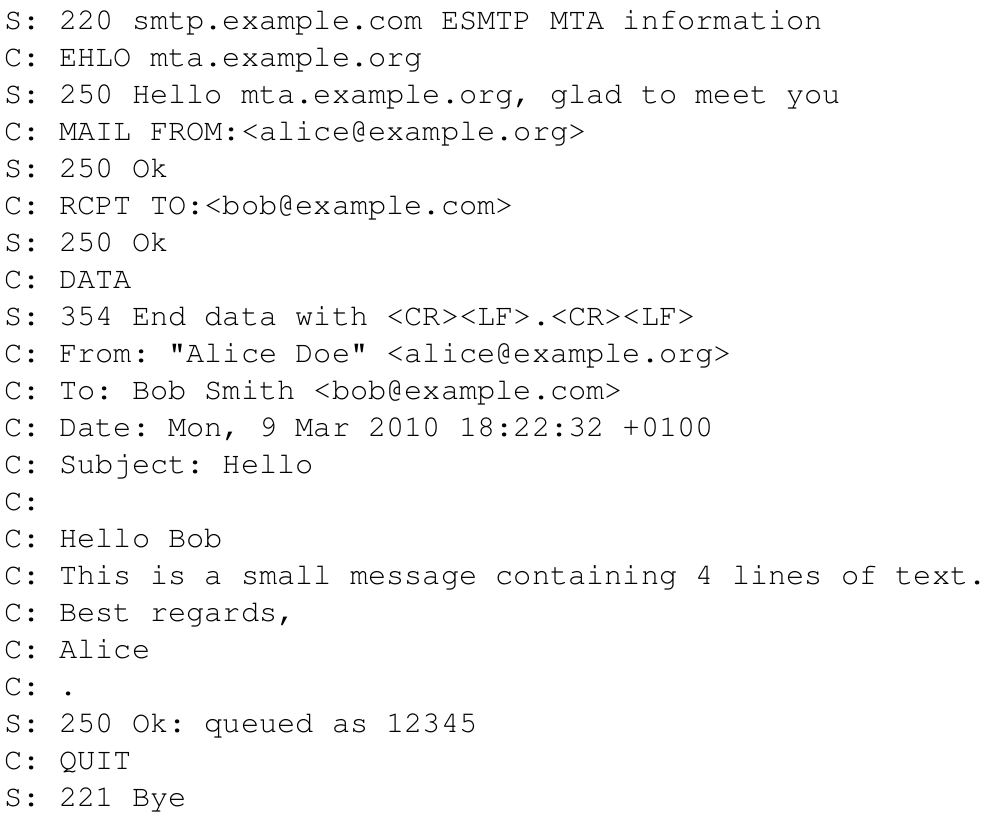
\includegraphics[width=7cm]{stmp.png} \\
\multicolumn{2}{m{15cm}}{220 : service ready, 221 : connection close, 250 : action okay, 354 : start mail, 3xx : need more information, 5xx : error}
\end{tabular}

\subsubsection{The post office protocol (POP) }
POP run above a connection-oriented service. (\textit{Server listen on port 110}), it allows a client to download all of his/her email from a server.

\paragraph{Working} :

\begin{tabular}{m{9cm}m{6cm}}
\begin{enumerate}
    \item Autorisation phase when the server verifies the client's credential 
        (\textit{username/password})
    \item Transaction pahase when the clien download message
    \item Update phase that conclude the session
\end{enumerate}
&
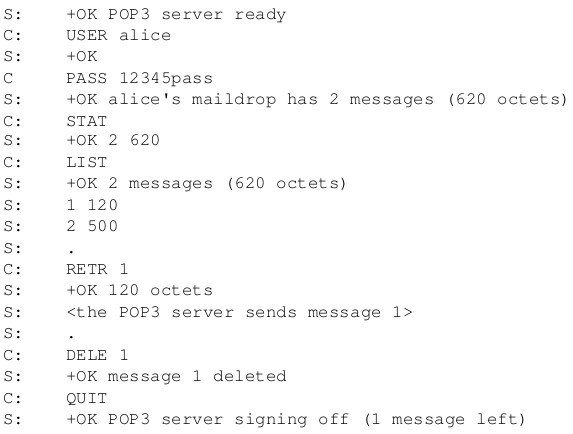
\includegraphics[width=7cm]{pop.png} \\
\multicolumn{2}{c}{+ok : accept, -ERR : error}
\end{tabular}


\subsection{HTTP}
Utilise des liens hypertext pour lier un fichier à un autre.

\paragraph{Trois composant du \textbf{World Wide Web}}
\begin{enumerate}
    \item \textbf{Uniform Resource Identifiers} : URI désigne une ressource sans aucune ambiguité
sur le world wide web.
    \item A standard document format : \textbf{HTML} contenant des liens hypertext
    \item A standard protocol with efficient acces to document on the server :\textbf{HTTP} composé de request (\textit{method, header, MIME document}) et response(\textit{status line, header, MIME document}).
\end{enumerate}

\paragraph{\textbf{URI}} est composé de 3 parties :
\begin{enumerate}
    \item A \textbf{protocol} for the application layer (http://, mailto:, ftp://)
    \item \textbf{Autorithy} wich is th IP adress or DNS server where is the file
    \item A \textbf{path} to the file in UNIX format
\end{enumerate}

\paragraph{\textbf{HTML}} 
Composed by two part : head and body.

\paragraph{\textbf{HTTP}}
Protocol is a text-based and run above a connection-oriented service. Contains :
\begin{enumerate}
    \item A \textbf{method} (\textit{GET, HEAD, POST}), a \textbf{URI} and version of HTTP protocol
    \item A \textbf{header} (specify optionnal parameter)
    \item An optionnal MIME
\end{enumerate}

\subparagraph{Persistent TCP connection}
Une requête \textsc{http} doit être \textbf{self-content}. C'est pour cette
raison que HTTP1.0 ouvrait une connection différente pour chaque requête HTTP.
HTTP1.1 ajoute les \textbf{persistent TCP connection} via
deux nouveau HTTP header :
\begin{itemize}
    \item \textbf{Connection} : with \textit{Keep-alive or close} to specified what 
        the client want
    \item \textbf{Keep-alive} : with the \textbf{maximum number} of request that the server
        agrees to serve and the \textbf{timeout} after wich the server will close an idle connection
\end{itemize}

\paragraph{Preferences}
Cependant, il est possible que le serveur veulent personnaliser les réponses au préférence du client. Trois solution :

\begin{enumerate}
    \item En forçant le client à s'identifier (user/password is deprecated)
    \item En utilisant des HTTP header tel que Accept-* . En pratique c'est pas utilisé
        sauf pour Accept-language par le naviguateur
    \item En utilisant des cookies via deux header : Cookie (\textit{request}) et 
        Set-cookie (\textit{response})
\end{enumerate}

\subsection{Remote Procedure call}
C'est comme appelé une procédure dans un code, sauf que l'on est pas sur
un host seul mais dans le réseau.

\paragraph{Encoding data} Le premier problème est d'encoder les données.
Deux mécanismes populaires existe :
\textsc{xdr} (\textit{plus efficace}), \textsc{json} (\textit{plus lisible}),\ldots

\paragraph{Reaching the call}
Le deuxième problème est d'envoyer les données.

Un mécanisme simple est \textsc{json-rpc} qui peut être utilisé en connectionless ou
connection-oriented, contenant :
\begin{itemize} 
    \item d'une requête : a string \textbf{jonrpc} indicant la version du protocol,
        le nom d'une \textbf{method}, une structure contenant les \textbf{params}
        et une \textbf{id}
    \item d'une réponse : a string \textbf{jonrpc} indicant la version du protocol,
        le \textbf{résultat} ou une erreur et l'\textbf{id}.
\end{itemize}


\subsection{Internet transport protocols}
In the internet, network layer provides a unreliable connectionless service and IP
adress to identifie each host, with
a maximun size packet equal to $64KBytes$ of payload.

\subsection{The User Datagram Protocol (UDP)}
C'est un unreliable connectionless transport service, au dessus d'une unreliable
connectionless network service, qui utilise les ports
pour permettre de communiquer avec plusieurs application et qui a comme
caractéristique :

\begin{itemize}
    \item SDUs doit être < 65467bytes
    \item Garantit pas que le SDU est délivré
    \item Ne peut pas délivré un SDU corrompu
\end{itemize}

\paragraph{Header} = Source port (16), dest port (16), length (16) et checksum (16)

\paragraph{Port} : 0 - 1023 (\textit{privileged}), 1024 - 49 151 (\textit{registered}),
49 152 - 65 535 (\textit{ephemere})

\paragraph{Utilisation} 
\textbf{UDP} is use when delay must be minimised or losses can be recovered by the application
itself. (\textit{Or real-time application like interactive video})


\subsection{The transmission control protocol (TCP)}
Bi-directionnal bytestream d'une connection-oriented transport service, au dessus d'une unreliable connectionless network service.

(Window-based transport protocol using go-back-n)

\paragraph{Header} :
\begin{itemize}
    \item Source adresse/port (16), dest adresse/port (16)
    \item sequence number per byte (32), ack number (32), window size (16)
        \begin{itemize}
            \item[$\to$] TO make a reliable data transfert
        \end{itemize}
    \item Flag : \textit{SYN, FIN, RST, ACK}
    \item checksum (16)
    \item Length in world (4)
\end{itemize}

\subsubsection{TCP connection etablishment}
Three-way handshake utilisant sequence number, ack number et SYN/ACK/RST flag.

\begin{figure}[!ht]
  \centering
  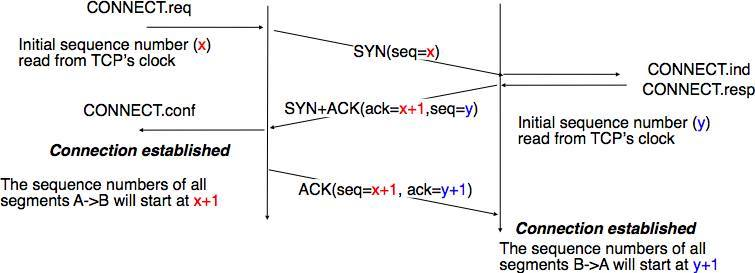
\includegraphics[width=12cm]{tcpconnect.jpg}
  \caption{Connection TCP}
  \label{fig:tcpconnect}
\end{figure}

Durant l'établissement de la connection, le client/serveur negocie plusieurs options :
\begin{enumerate}
  \item Le \textbf{MSS} qui est la taille du plus grand payload acceptable (\textit{536 au minimun})
  \item La taille de la window
  \item L'utilisation de SACK (information sur segments reçu hors séquence)
  \item Un ensemble d'option où client/server disent respectivemnt ce qu'il veut et ce
    qu'il supporte
\end{enumerate}

\paragraph{Encodage des options} est fait en \textsc{TLV}, Type Length Value.

\paragraph{Robustness principe} : On peut recevoir dans SYN des options que l'on
comprend pas sans crasher, toutefois dans SYN+ACK on ne répond que par ce
que l'on connait.

\paragraph{Denial of service attacks}
Un serveur maintient un TCB (transmission control block) qui contient 
les état des TCP entity pour chaque connection. Pour éviter un overflow
de la mémoire, la taille du TCB est limité à 100.

La \textbf{Denial of service attacks} essaye de rendre une donnée 
sur le réseau non disponible.

\textbf{SYN flood attack} a juste a surcharger le serveur de SYN
pour surcharger son TCB et empecher tout le monde d'établir une connection avec
lui.

\subparagraph{Solution :} Utiliser un cookie chez le client
pour remplacer la TCB sur le serveur. Toutefois, il n'est pas
totalement compatible avec TCP option.

\subsubsection{TCP reliable data transfert}

Pour chaque connection TCP, on maintiens un \textbf{TCB} (transmission control block)
avec toute les informations nécessaire pour envoyer et recevoir des segments.

\paragraph{Segment transmission strategie}

Deux solutions extrêmes :
\begin{enumerate}
    \item Envoyer quand on a besoin, mais cela peut impliquer d'envoyer
        un byte d'information avec 20 byte d'header\ldots pas très efficace
    \item L'autre extreme est d'envoyer qd on a rempli \textsc{mss} byte of data
\end{enumerate}

\subparagraph{Nagle  algorithm}  :   on  envoi  le  paquet   si  il  rempli
un  \textsc{mss}  ou  si  l'on  vient  de  recevoir  un  acknwoledgement
(\textit{càd au moins à chaque round trip time}).

\subsubsection{TCP window}

La négociation du  window scaling factor ($0 \leq scaling  \leq 14$) se
fait  à la  connection, même  si certaines  implementations permettent
d'automatiquement ajuster la taille.

\subsubsection{TCP retransmission}
\textbf{Go-back-n} a besoin d'un bon timer de retransmission (\textsc{rtt} est une
bonne estimation même si il change pdt la connection)
\begin{center}
\textsc{rtt} $\approx$ delai entre la transmission d'un segment et la reception de l'ack
\end{center}

\paragraph{Measure RTT }
Le problème est que l'on ne sait pas de quel segment l'ack est la réponse (càd qu'il pourrait
y avoir plusieurs segment identique envoyé)

Pour cela on utilise le \textbf{timestamp option} :
\begin{itemize}
    \item \textbf{TS} : Par exemple valeur de la clock
    \item \textbf{TS} echo : Dernier \textsc{ts}val reçu
\end{itemize}

Comme y'a plus d'ambiguité, on peut mettre à jour la valeur du time ( rtt = 3 sec à l'initialisation).
\begin{eqnarray*}
srtt \textrm{ (smoothed rtt mcomputed) } &=&  (\alpha \times srtt) + (1-\alpha) \times rtt) \\
rto \textrm{ (retransmission timedout) } &=& min(60, max(1, \beta \times srtt))
\end{eqnarray*}

où rtt est le RTT mesuré et 1-60 sont les bornes minimal/maximal.


\subparagraph{Jacobson's algorithm} : en pratique ça marche pas bien, donc jacobson a une
autre idée. rto est toujours initialisé à 3 sec.
\begin{multicols}{2}
\begin{itemize}
    \item[-] Pour la première valeur de RTT
        \begin{eqnarray*}
            srtt &=& rtt \\
            rttvar &=& var / 2 \\
            rto &=& srtt + 4 * rttvar 
        \end{eqnarray*}

    \item[-] Ensuite
        \begin{eqnarray*}
        rto &=& srtt + 4*rttvar \\
        rttvar &=& (1-\beta) \times rttvar + \beta \times |srtt - rtt| \\
        srtt &=&  (\alpha \times srtt) + (1-\alpha) \times rtt) 
        \end{eqnarray*}
\end{itemize}
\end{multicols}

\paragraph{$\alpha, \beta$ value : }  $\beta = \frac{1}{4}, \alpha = \frac{1}{8}$

\subsubsection{Advanced retransmission strategie}

\paragraph{}
\textsc{tcp} utilise de base \textbf{go-back-n}, et lorsque le même timer
expire on recommande de doubler le timer (appellé \textit{exponential backoff}) jusqu'à
ce qu'il ait atteint 60sec où le host est considéré inateignable.

\paragraph{Piggybacking} est utilisé par TCP lorsque il y a un échange de 
donnée bi-directionnel, ce qui reste plutôt rare.

\paragraph{delayed acknowledgement strategy}
Par ailleurs, il est aussi possible de perdre bcp de performance en envoyant des
ack quand il n'ont pas bcp d'interet. Typiquement, il est possible d'implémenter
un \textbf{delayed acknowledgement strategy} qui assure d'envoyer un ack a chaque fin
de timer (\textit{delai cour souvent d'une seconde}) ou si il reçoit un segment hors séquence puisque du coup
l'ack a énormément d'importance

\paragraph{Out-sequence}
Il est très facile pour le receiver d'ajouter un buffer pour récupérer les
segments hors séquence sans avoir besoin d'en informer le sender.

\paragraph{Fast retransmit}
Actuellement, lorsqu'un segment est perdu il faut attendre que son timer expire
pour pouvoir le renvoyer. Une autre méthode consiste à détecter l'erreur lorsque
l'on reçoit 3 ack portant sur le même segment.

Il nécessite l'ajout d'une variable dubpacks dans le \textsc{tcb}.

\paragraph{Selective repeat}
Avec une option de TCP, on peut activer les \textbf{SACK} qui permettent d'indiquer
les segments qui ont été reçu hors séquence. On utilise ici souvent Fast retransmit avec.

\subsubsection{TCP connection release}
Abrut (\textsc{rst}) ou gracefully (FIN, FIN+ACK)

\subsection{The stream control transmission protocol (SCTP) }
Alternative au TCP qui offre :
\begin{enumerate}
    \item Supporte efficacement the \textbf{multihomed host} càd avec plusieurs interface réseau. En TCP, une IP par interface et si tu te connecte en WifI puis que ça
        crash la connection ne sait pas être reprise par la 3G.
    \item La possibilité de pouvoir envoyer des \textbf{messages} par bytestream
    \item Partially-reliable, usefull for timed delivery
    \item Une seule vrai connection avec des streams \textit{logique} pour éviter de manager
        plusieurs connection
\end{enumerate}

\subsubsection{Segment}
C'est un header suivit d'un ensemble de chunk.
\begin{figure}[h]
    \centering
    \begin{tabular}{m{8cm}m{7cm}}
        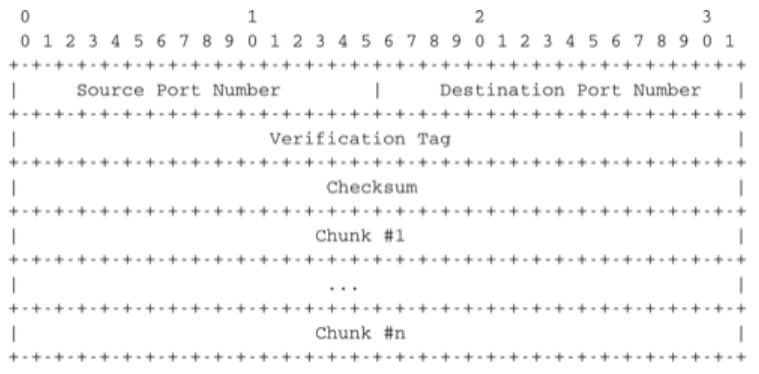
\includegraphics[width=8cm]{sctpsegment.png} &
        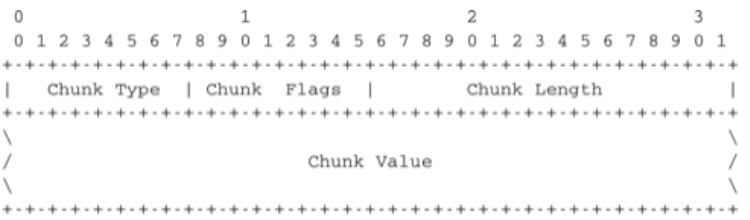
\includegraphics[width=7cm]{sctpchunk.png}
    \end{tabular}
    \caption{SCTP segment/chunk format}
\end{figure}

\paragraph{Header} = Source port number (16), dest port number (16), verification tag (32) and checksum (32).

\paragraph{Chunk} = Type (8), flags (8), length (16) et value (32) pour permettre d'insérer facilement un ensemble d'option. 
STCP, contrairement à TCP, n'est pas limité sur le nombre d'option. C'est bon exemple de format de protocol facilement etendable.
 

\subsubsection{Connection etablishment}
C'est un four-way handshake (pour contrer l'attaque ``Denial attack service'')

\begin{figure}[h]
    \centering
    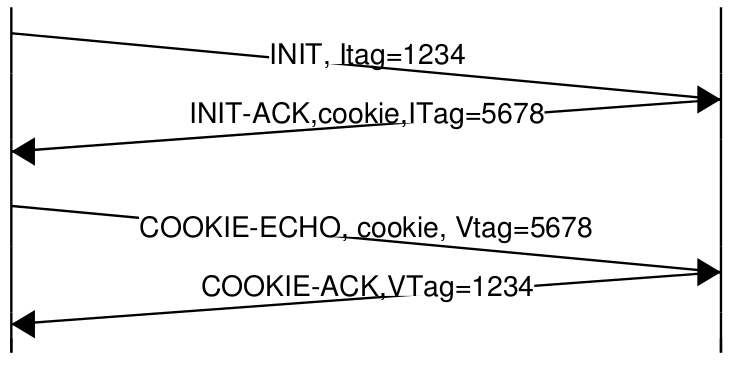
\includegraphics[width=6cm]{fourway.png}
    \caption{Fourway handshake}
\end{figure}

\subsubsection{Reliable data transfert}

\begin{figure}[h]
    \centering
    \begin{tabular}{m{8cm}m{8cm}}
    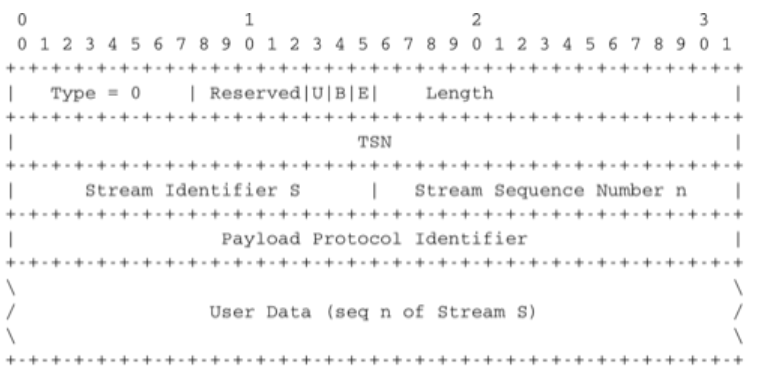
\includegraphics[width=8cm]{datachunk.png} &
    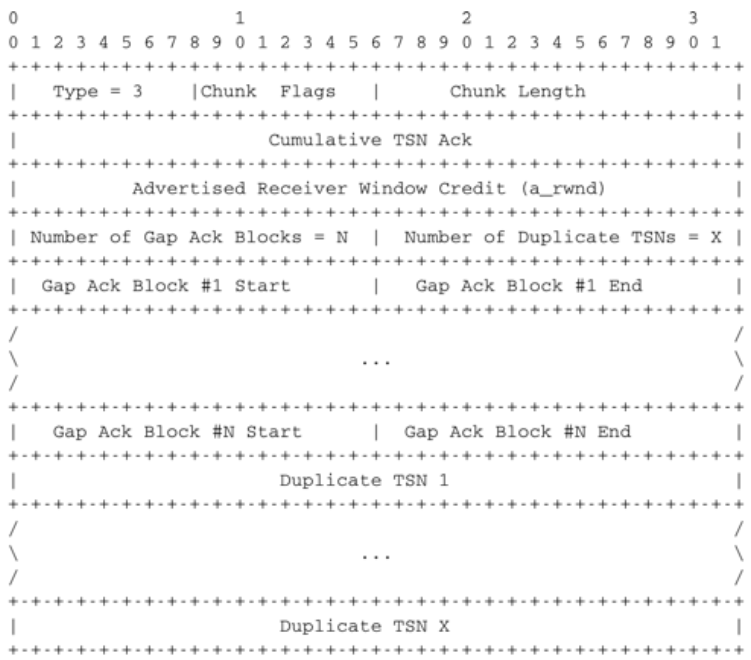
\includegraphics[width=8cm]{sackchunk.png} 
\end{tabular}
    \caption{SCTP data/sack chunk format}
\end{figure}

\paragraph{Data chunck}
Les données sont envoyé via des \textbf{data chunck} qui utilise un TNS comme
numéro de séquence (augmenter de 1 a chaque data chunck). Lorsqu'un chunck est
scindé on utilise le bit \textsc{b} et \textsc{e} pour spécifier le premier et dernier
chunck.

\paragraph{Sack chunk}
Pour garantir l'arrivé, un TNS ack cumulatif est utilisé (Is on chunck level and not
byte level). Il donne aussi des informations sur les chunck hors séquence.
Plusieurs autre différence :
\begin{enumerate}
    \item Il peut fournir de l'information sur \textbf{LES} différents ``trou'' dans le buffer de réception
    \item Il peut donner un feedback sur chunck dupplicate (Annonce une mauvaise heuristic du sender)
\end{enumerate}

\subsubsection{Connection release}
Applique un three-way handshake pour cloturer la connection, ou un ABORT chunk
pour refuser une connection ou la cloturer immédiatement.

\subsection{UDP - TCP - SCTP}
\begin{table}[h]
    \begin{tabular}{|c|c|c|c|c|c|}
    	   \hline
    	    Protocol& Reliablility&\#options&Mode&Establishment&Num seq\\
        \hline
        UDP & Unreliable   & x              & Stream-mode     & x                   & x \\
        \hline
        TCP & Reliable     & Option finie   & Stream-mode     & Three-way handshake & seq. = byte \\
            &              &                &  Single host    &                     &  \\
        \hline
        SCTP & reliable or & Option infinie & message mode as & Four-way handshake & chunk \\
             & partially   & with chunk     & a stream mode   &                    & \\
             &             &                & Multihomed host &                    & \\
        \hline
    \end{tabular}
    \caption{Difference between UDP, TCP and SCTP}
\end{table}
\subsection{Congestion control}
Le control est effectué dans la transport layer.

\textsc{tcp} control la congestion en agissant sur la window size puisque une connection
ne peut pas envoyer des données plus vite que  $$\frac{window}{rtt}\quad window=min(swin,rwin)$$

\paragraph{Congestion window}
\textbf{CWND} est stocké dans le \textsc{TCB} de chaque connection, et la taille de la window
est $min(cwnd, rwin, swin)$.  
\begin{itemize}
    \item[-] \textit{Additive increase} : Chaque \textsc{rount trip time}, on incremente \textsc{cwnd} de MSS byte. (congestion avoidance phase)
    \item[-] \textit{Multiplicative decrease} : Quand une congestion
est detecté on divise \textsc{cwnd}.
\end{itemize}

\paragraph{Initial value cwnd}
est de \textbf{MSS} bytes afin de ne pas congestionner le réseau au démarrage.
(Cette valeur de départ a été augmenter à 15Kbyte)


Toutefois, cwnd va augmenter lentement avant d'arriver a une valeur qui utilise efficacement le
reseau. Pour éviter cela, on inclu un \textbf{slow-start algorithm} qui permet durant ce temps
de doubler \textsc{cwnd} chaque RTT.

\paragraph{Detect congestion} revient à detecter la perte de packet.
\begin{itemize}
    \item \textit{mild congestion} : Si on effecture un fast retransmit (on divise cwin par 2)
    \item \textit{severe congestion} : Quand le timer de transmission expire (on divise sstresh par 2 et cwin =MSS)
\end{itemize}

\begin{figure}[h]
    \centering
    \begin{tabular}{m{8cm}m{8cm}}
    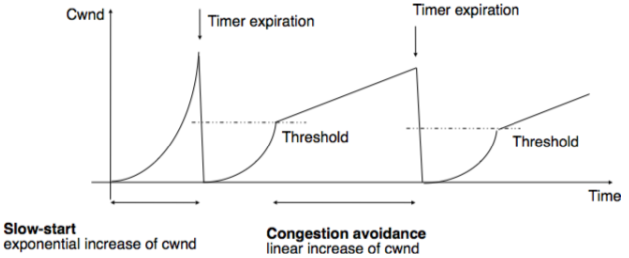
\includegraphics[width=8cm]{severecongestion.png} &
    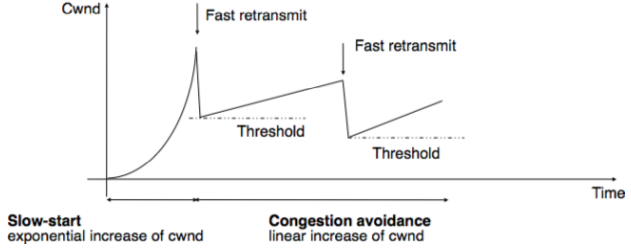
\includegraphics[width=8cm]{midlecongestion.png} \\
    \multicolumn{1}{c}{Severe congestion} & \multicolumn{1}{c}{Middle congestion }
\end{tabular}
    \caption{Congestion window when detect congestion}
\end{figure}

\subsubsection{Controlling congestion without losing data}
L'idée est de détecter avant la perte de paquet la futur congestion avec un
\textbf{Explicit Congestion Notification}. (Quant un paquet passe par un router
congestionné on met le \textbf{CE} bit à 1 et quand le receiver à cette information il la
transmet au sender pour adapter son débit)

\begin{enumerate}
    \item Pour déployer la solution, il faut un \textbf{autre bit} (ECT,ECN-capable transport) pour spécifier si le packet utilise
        \textbf{ECN} ou non. En effet, le cas échéant lorsque le router est congestionné ceux qui
        n'implémente pas ECN sont avantagé.
        \begin{itemize}
            \item[$\to$] Si le router est congestionné et que le packet implémente ECN alors CE est mis à 1, sinon le packet est discard.
        \end{itemize}
    \item Si le protocol est reliable ont peut informer le sender via l'ack. Soit via
        un flag dans le header soit via une option. (TCP=flag, STCP=option).
        \begin{itemize}
            \item[$\to$] Une variable est maintenue à 1 du coté du receiver tant que 
                les paquets reçu sont marqué comme ``congestionné''.
        \end{itemize}
    \item Dernièrement, le sender/receiver savent si il utilise ECN via une TCP option
        durant le three-way handshake de connection
\end{enumerate}

Si le receiver detect une congestion, les prochain paquets envoyé auront cette information.
(Pour éviter que l'information ne se perde si l'ack est perdu)

\paragraph{Router algorithm}
Deux types de router, soit avec une FIFO soit un ensemble de FIFO et round robin scheduler.

Au lieu de prendre une mesure instantanée du remplissage du buffer, on prend une moyenne
du remplissage.
De plus, chaque paquet à une probabilité d'être marqué comme congestionné qui augmente
quand la moyenne augmente. (Random Early Detection)

\paragraph{}
Quand il y a plusieurs queue ont fait cette probabilité de manière indépendante pour
garantir la justesse.

\subsubsection{Modeling TCP congestion control}
To show the factors that affect the performance of TCP,
if $p$ is the segment loss ratio then $\frac{1}{p}$ is the number of segment successfully transfers.

\begin{figure}[h]
    \centering
    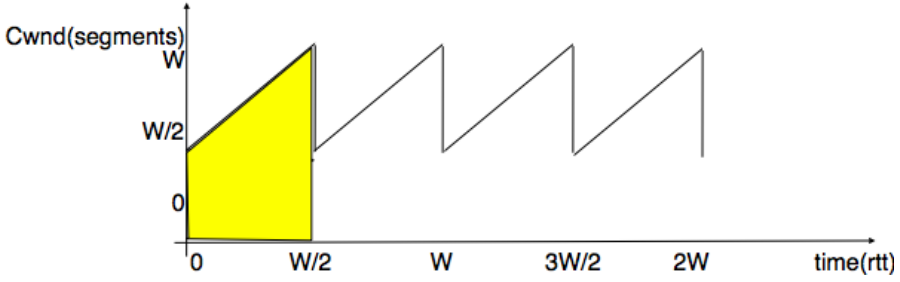
\includegraphics[width=9cm]{modelingtcp.png}
    \caption{Evolution of the congestion window with regular losses}
\end{figure}

\begin{description}
    \item The number of segment that are sent during a cycle is the yellow : 
    $ area = \frac{3 \times W^2}{8}$
    \item But by definition, area = $\frac{1}{p}$ so : $ W = \frac{k}{\sqrt{p}}$
    \item The troughput (\textit{bytes/sec}) is the number of segment transmitted divided
        by the duration of the cycle : $$Throughput = \frac{area \times MSS}{time} \quad \approx \frac{k \times MSS}{rtt \times \sqrt{p}}$$
\end{description}

This is a important result wich show that :
\begin{itemize}
    \item TCP connection with \textbf{small rtt} higher throughput that higher rtt
        when losse occur. (\textit{unfair})
    \item TCP connection that use \textbf{large MSS} can achieve a higher throughput that
        shorter MSS. (\textit{unfair}). Note that most host use same MSS = 1460 bytes.
\end{itemize}

\paragraph{Conclusion :} $Througput < min( \frac{window}{rtt}, \frac{k \times MSS}{rtt \times \sqrt{p}})$
Maximun throughput depend on the maximun window size and rtt if there are no losses,
else it depends on the MSS, rtt and loss ratio.

\subsection{Network layer}
Trois type de datalink layer :
\begin{enumerate}
    \item Directement un lien physique du physical layer
    \item Local Area Network
    \item Non-Broadcast Multi-Access (utilisé pour simuler une LAN supportant
        juste l'unicast)
\end{enumerate}

\paragraph{LAN} Dans une LAN Chaque host est identifié par une adresse datalink layer
(\textbf{MAC adresse}).

LAN supporte broadcast and multicast datalink layer adresses. Une frame envoyé a l'adresse
\textbf{multicast} de la LAN est envoyé à tout les participants correspondant
au groupe. L'addresse \textbf{broadcast} est utilisé piur envoyer des messages à tout le monde. 

\subsubsection{IP version 6}
IPv4 ne pourra bientot plus supporter toute les adresses, d'ou le besoin
de passer à une autre solution.

\begin{tabular}{m{2.5cm}m{10cm}}
    Assumptions : &
    \begin{itemize}
        \item[-] Adress encoded on 128 bits
        \item[-] IPv6 format header easily be parsed by hardware device
        \item[-] Able to configure IPv6 adress automatically
        \item[-] Security
    \end{itemize}
\end{tabular}
    
\paragraph{IPv6 adressing architecture}
Scalability of a network layer protocol depend on its addressing architecture.

IPv6 support \textbf{unicast, multicast and anycast}.

\paragraph{\textbf{Unicast}} :

\begin{tabular}{m{8cm}m{7cm}}
    \begin{itemize}
        \item Global routing prefix that assigned to the \textbf{Internet Service Provider}
        \item Subnet id identifies a customer of ISP
        \item Interface id
    \end{itemize}
    &
    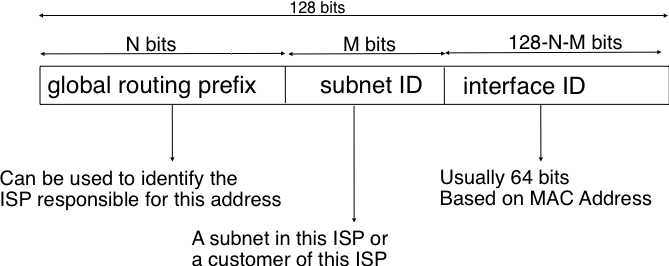
\includegraphics[width=8cm]{unicast.png}
\end{tabular}

\paragraph{ }
Une allocation \textbf{hierarchique} des allocations d'adresse permet de minimiser
le nombre de route connu par les router. Celui ci connait donc la route pour
certains block d'adresse!
(\textit{$2^{128}$ groupé dans $2^{64}$ subnet!})

Deux type d'allocation d'adresse :
\begin{itemize}
    \item \textit{provider independent} (PI) : Pour compagnies connecté a au moins deux ISP. 
        Ca correspond à recevoir un \textbf{block d'adresse} indépendant du ISP.
    \item \textit{provider aggregatable} (PA) : Est dépendante du provider.
\end{itemize}

Le désavantage des \textbf{PA} adresses est que lorsque tu utilises un block d'adresse PA
et que le provider change, il change aussi toute les adresses utilisés.

\paragraph{Size IPv6 adress}
/32 = Internet Service Provider, /48 = single compagny, /56 = small user site,
/64 = single user, /128 = rare (Pas plus d'un host attaché au prefix)

\paragraph{Utilisation IPv6 prefix}
\textbf{Longest prefix match} assure que la route qui match le plus avec
l'adresse est celle qui est employé.

Note : ::/0 match avec tout le monde et est donc la \textit{default route}.

\paragraph{\textbf{Unique Local Unicast}}
L'adresse ULA est un fc00::/7 et est similaire à une IPv4 adresse.
L'adresse n'est pas garantie unique et un router ne forwarde pas
une ULA.

Note que contrairement au link local unicast, celle ci ne doit pas forcément
avoir le même lien.

\paragraph{\textbf{Link Local Unicast}}
L'addresse commence par fe80::/64 et est suivi des 64 bits d'interfaces.
Utilisé quand deux host sur le même lien (or LAN) veulent échanger des
packet.. Note que le router ne peut pas forwarder un packet avec un
link local unicast.

(\textit{Utilisé qd on ne peut pas avoir une IPv6 régulière, càd en LAN isolé})

\paragraph{\textbf{Multicast}}
Permet d'envoyer un packet à toute les personnes d'une même groupe, dans une LAN.

\begin{figure}[h]
    \centering
    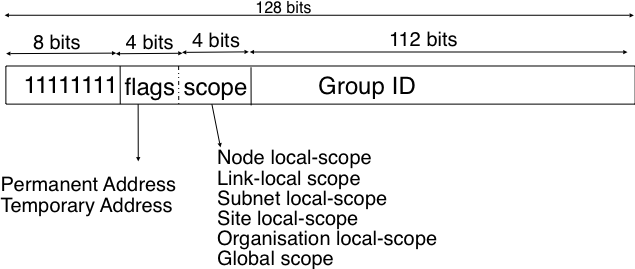
\includegraphics[width=8cm]{multicast.png}
    \caption{Multicast adress}
\end{figure}


\paragraph{\textbf{IPv6 packet format}}

\begin{figure}[h]
    \centering
    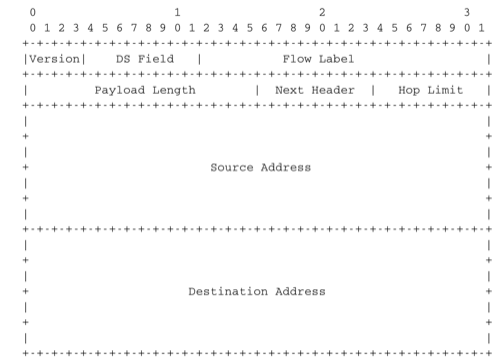
\includegraphics[width=12cm]{ipv6format.png}
    \caption{IPv6 packet format}
\end{figure}

\subparagraph{Header}(40bytes) = Payload length (16 bits), Hop limit : \textit{limit of router
that can forward the packet} (8 bits) et Next header (8bits)+Version(4bits)+
SRC(128b)+DST(128b)+Traffic(8 bits ECE/ECT).

\subparagraph{No checksum}
Il n'y a pas de checksum dans le header de packet IPv6 car il y a déja le checksum
sur les \textbf{frames} au niveau datalink layer! En pratique, l'ajout d'un tel checksum prévient
les erreur de corruption de mémoire au sein d'un routeur (\textit{ridicule}) pour un coùt de
calcule élevé.

\subparagraph{Next header}
Indique le prochain header, tel que un transport layer header (\textit{UDP=17, TCP=6, SCTP=132}) ou une IPv6 option car les paquets peuvent avoir plusieurs header. Note qu'une option a aussi le champ \textit{next header}.

\subparagraph{Options}
Contiennet un next header, une length et un \textbf{opt field} qui indique
ce que le receiver doit faire si il ne reconnait pas l'option : 
\begin{itemize}
    \item[-] 00 : il continue sans se soucier de l'option
    \item[-] 01 : il supprime le packet
    \item[-] 10 : il retourne un packet de control
\end{itemize}

\subparagraph{Fragment option}
En IPv6 la fragmentation est fait par le sender et non par le router. (Celui-ci discard
le paquet et envoi un message d'erreur au sender si le packet est trop grand).

Un paquet fragmenté contient :
\begin{itemize} 
    \item[-] Offset (13) de la fragmentation
    \item[-] Next header (8) (\textit{car une option})
    \item[-] Un flag : 0 = dernier fragment,
    \item[-] Champ pour \textit{identifier} le packet original. Il faut être sur de ne pas utiliser le même pdt 
    une période de MSL secondes.
\end{itemize}

\subparagraph{Note:} On peut envoyer les packets du premier au dernier ou dans l'ordre inverse.
La deuxieme solution permet au receiver de connaître la taille du paquet (et donc du buffer
nécessaire). Quand un fragment, on lance un timer, si tout les fragment ne sont pas arrivé à la fin du 
timer, alors le paquet est considéré comme perdu.
\paragraph{Loose source} Option IPv6 pour préciser la routes à prendre (on spécifie l'addresse des routeurs). Pas utilisé car problème de sécurit'é.

\subsubsection{ICMP version 6}
\textit{Internet Control Message Protocol} version 6 est utilisé dans un paquet IPv6
(next header = 58) pour transmettre des messages au sender. Deux type de messages :

\begin{itemize}
    \item Messages d'erreurs
        \begin{enumerate}
            \item Destination unreachable (0: no route, 1: firewall refuse, 2: sender use link-local adresse to reach global unicast adresss, 3: adress unreachable, 4: port unreachable)
            \item Packet too big
            \item Time exceeded
            \item Parameter problem
        \end{enumerate}
    \item Messages d'information : Lorsque qu'un host reçoit un \textit{Echo request},
        il doit répondre avec un \textit{Echo reply}.
\end{itemize}
\paragraph{PathMTUDiscovery} Use of ICMP segment to discover the MTU of the path. Then adjust MSS to avoid fragmentation.

\subsection{The IPv6 subnet}

Chaque interface sur un device est identifié par une MAC adresse unique. \footnote{MAC adress block are allocated to manufacturers}.

Grace à cette unicité, deux hosts connecté sur une LAN a donc une adresse unique!

\paragraph{Broadcast :} le packet est délivré à tout les devices attaché au datalink network
\paragraph{Multicast :} On fait un broadcast sauf que l'interface du device sait si le
packet lui est destiné ou non (\textit{sur base d'une adresse logique}).

Potentiellement, tout les node IPv6 sont capable de captuer des frames destinés à different
autre multicast adresse.

\subsubsection{Interactions between IPv6 and datalink layer}

\paragraph{Dans une LAN  sans internet}, les hosts prennent une  adresse IP grace au
\textbf{link-local adresse} : on prend fe80::/64 avec la MAC adresse.

\paragraph{Si  la  LAN  est  connecté à  internet},  on  utilise  \textbf{Neighbor
Discovery  Protocol} (partie  de ICMPv6)  pour connaître  l'adresse des
autres

\paragraph{Neighbor Discovery Protocol (NDP)}
Attention les addresses IPv6 ont été configuré manuellement.
\begin{enumerate}
    \item Envoi un multicast \textbf{ICMPv6 Neighbor Solicitation} (NA) avec l'adresse IPv6 recherché
    \item Le receiver répond avec un \textbf{ICMPv6 Neighbor Advertisement} avec son adresse IPv6 et MAC
    \item En recevant le ICMPv6 NA, il stock le lien IPv6-MAC dans sa \textbf{NDP table} (Mapping between IP address and MAC )
\end{enumerate}

\subparagraph{Note:} ICMPv6 NS peut aussi être utilisé en unicast pour voir si un host est atteignable. 
De plus, le ICMPv6 NA est stocké temporairement dans la cache et quand il expire il faut revalider l'adresse.

\paragraph{Duplicate Address Detection algorithm} permet de ne pas avoir deux adresses IPv6
identiques.
Pour cela il envoit un \textbf{ICMPv6 NS} en unicast à sonn adresse, et si il ne reçoit pas de réponse elle est donc unique.

\paragraph{\textbf{Automatically configure IPv6 adress}}
There is two protocol : SLAAC and DHCPv6.

\subparagraph{Stateless Address Auto-Configuration (SLAAC) }
\begin{enumerate}
    \item Un device crée sa \textbf{link-local adresse} avec fe80::/64 et 64bits 
        issus en partie de MAC
    \item Il vérifie son unicité en envoyant un \textbf{ICMPv6 NS} avec son link-local en multicast
    \item Pour connaître le \textit{prefix IPv6 subnet}, le router envoi
        régulièrement des ICMPv6 \textbf{Router Advertisement} multicast sur
        \textbf{ff02::1} \footnote{Correspond à tout les hosts disponible} contenant : 
        \begin{itemize}
            \item[-] \textit{Cur hop limit} : Maximun intermediare router (souvent 64)
            \item[-] \textit{Router lifetime} : Temps estimé ou le router est le router par
                défault
            \item[-] \textit{Reachable time and Retrans timer} : utilisé pour configuré 
                l'utilisation du NDP protocol pour les hosts du subnet
        \end{itemize}

        Beaucoup d'\textbf{option} peuvent être pacer dans Router Advertisement messages :
        \begin{itemize}
            \item \textbf{MTU} option : Indique la taille maximun de ce qui peut être
                transmit \textbf{sans} fragmentation sur le subnet
            \item \textbf{Prefix} option : Donne la taille du prefix et sa length, ainsi que la 
                durée de vie estimé du préfix.
        \end{itemize}           
    \item IPv6 adresse = Prefix + 64 bits d'identification
    \item Envoi un \textbf{ICMPv6 NS} a son adresse IPv6 pour s'assurer de l'unicité
\end{enumerate}

\subparagraph{Notes:} Un device peut envoyer un ICMPv6 Router Solicitation au router
via \textbf{ff01::2} \footnote{Correspond à tout les routers disponible} pour
demander un ICMPv6 RA si il considère le délai trop long.


\subparagraph{Dynamic Host Configuration Protocol (DHCP)}
Utilise un serveur DHCP. Ce serveur a un ensemble d'addresse et écoute sur le port 67.
\begin{itemize}
	\item Quand un host se connect, il envoie un \textbf{DHCP request} en UDP à tout les serveurs DHCP
	\item Le serveur capture la request, et envoie un \textbf{DHCP reply} avec un addresse IP non assigné. 
	Ce reply contient aussi le temps de vie de l'addresse pour forcer à renouveller son addresse.(Donc les addresse peuvent être réutilisé).
\end{itemize}

\paragraph{Multi router on subnet}
Grace au \textbf{ICMPv6 Redirect Message}, il est possible que les hosts
apprennent automatiquement les nouvelles routes :

\begin{itemize}
    \item[-] Lorsque un router doit forwarded back un packet, il envoit un
ICMPv6 RM qui indique que le packet doit être envoyé par un autre router.

    \item[-] Celui ci met à jour sa forwarding table (\textit{timer est souvent associé 
    à ce nouveau router pour supprimer la router après un certain temps})
\end{itemize}


\subsection{Routing in IP networks}
Deux classe de protocol entre différents domaines pour echanger
efficacement de l'information.

Une grande différence entre \textbf{intra} et \textbf{inter} domaine est 
la \textit{routing policies} utilisé par chaque domaine.

Dans un domaine toute les routers sont égaux et la meilleur route est choisi sur
différents critére : temps, nombre d'intermédiare et taille de bandwith.

\subsection{Intradomain routing}
Echange des informations sur les destinations atteignables \textbf{dans} le domain.
\textit{RIP} est protocol de \textbf{distance vector} et \textit{OSPF} 
utilise \textbf{link-state routing}.

\subsubsection{RIP}
Les routers echanges periodiquement des RIP messages (inside \textbf{UDP} segment).

Pour accélerer le processus quand un router boot, il peut envoyer une 
\textbf{RIP request} en multicast à ff02::9
(\textit{pour demander les tables de routings}).  

Tout ceux qui reçoivent la demande répond en envoyant sa routing table avec 
une séquence de \textbf{RIP response}.

\paragraph{Note: } Les routers envoyaient périodiquement (30sec) une ou plusieurs RIP response
reprenant les distances vectors qui résume la routing table. Mais cela causait au routeur de se synchroniser et parfois d'être surcharger. Maintenant ils attendent un temps aléatoire entre 15 et 30.

\subsubsection{OSPF}
Avec le link-state routing, pour des grands réseaux c'est très couteux de stocker
l'ensemble du réseau en mémoire.

\begin{tabular}{m{10cm}m{5cm}}
    \begin{itemize}
        \item \textbf{Border router} : Router attaché à plusieurs area
        \item \textbf{Internal router }
        \item \textbf{Area} : Les routers connaissent la topologie de leur area
            et comment rejoindre la backbone area. 
        \item \textbf{Backbone area} : C'est l'area qui regroupe les \textbf{border
            router} et ceux qui ne sont pas dans une area.
    \end{itemize}
    &
    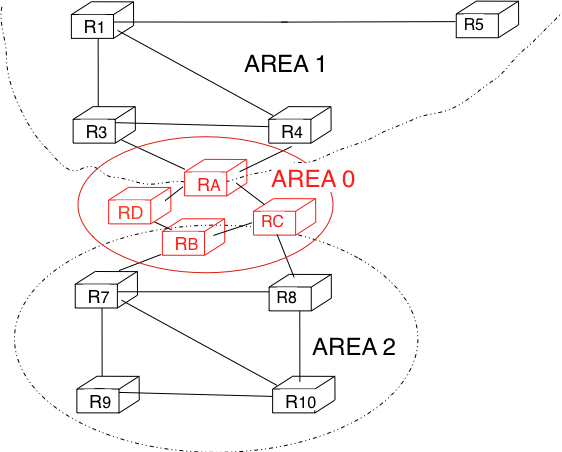
\includegraphics[width=5cm]{area.png}
\end{tabular}

\paragraph{Area} 
Les routers échangent des link-state packet à tout ceux dans l'area.

\paragraph{Inter-area}
L'inter-area  routing  est  fait  en  échangeant  des  distance  vector
protocol pour prévenir  les routeur d'une area le cout pour atteindre
un routeur d'un autre domain.

\paragraph{LAN}
Quand  les  routeurs  boot  dans   un  LAN,  ils  élisent  un  routeurs
(\textbf{Designated  Routeur}) pour  ne pas  devoir échanger  des HELLO  packet
entre tout  les routeurs. Les  routeurs peuvent seulement  échanger des
HELLO avec le DR : c'est lui qui représente la LAN.

(\textit{La  topologie  de  la  LAN   apparait  comme  un  full-mesh  of
point-to-point link connected to the DR router})

\subsubsection{Shortest path}
Les protocoles intradomaines choississent les plus court chemin. Il peut arriver qu'il y ait deux
chemins qui aient le même coût. Dans ce cas deux approches:
\begin{itemize}
    \item On utilise toujours le même (\textit{en ne mettant que celui la dans la forwarding table}).
	\item On utilise les différents chemin:
	\begin{itemize}
		\item Via un Round Robin mais cela implique d'utiliser des chemins différent pour les 			
		paquets d'un même flow (TCP connection) et potentiellemnt augmenter les arrivées
        hors séquence. 
        \begin{center}
            (\textit{hors-sequence $\to$ dupplicate ack $\to$ fast retransmit $\to$ congestion })
        \end{center}

		\item Utiliser un Round Robin par flow, via une hash value du tuple de paquet.
		   La même interface (chemin) sera utiliser pour les paquets du même flow.
            $$hash( NextHeader, IP_{src}, IP_{dst}, Port_{src}, Port_{dst} ) mod N$$
            N is the number or outgoing interface on the equal cost paths
	\end{itemize}
\end{itemize}

\subsection{Interdomain routing}
Echange de l'informations entre les domaines. Cette information est une information
agrégé des routers et on considère ici les domaines comme des boîtes noires.

A \textit{content-rich} sub domain is a domain that contains hosts that
mainly receive packets. (Google,\ldots)

\subsubsection{Connected link}
\begin{itemize}
    \item \textbf{Private peering link} permet de lier deux domaines. Pour des questions
de performances plusieurs lien physique sont établi entre les domaines.

     \item \textbf{Internet eXchange Point} Une solution moins couteuse est de les connecter
via un IXP.  The IXP contient une LAN où tout les routers sont connectés.
\end{itemize}

\begin{figure}[h]
    \centering
    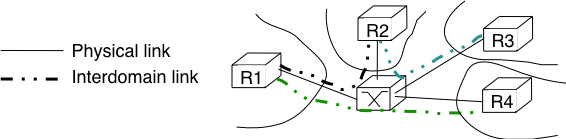
\includegraphics[width=8cm]{exchange.png}
    \caption{Internet eXchange Point}
\end{figure}

\subsubsection{Connection cost} 
Le \textbf{coût} d'une route est très importante en interdomain
alors qu'en intra on préfére la performance.

\begin{figure}[h]
    \centering
    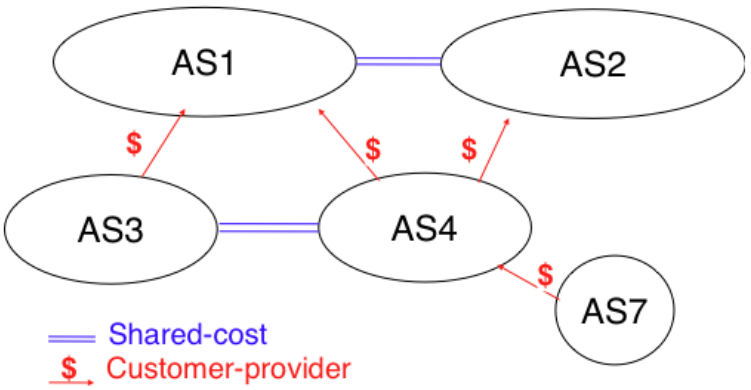
\includegraphics[width=5cm]{peering.png}
    \caption{Peering relationships}
\end{figure}

Il existe deux types de relation entre domaine
\begin{itemize}
    \item \textbf{customer->provider} :
        Le customer paye pour que son domaine soit distribué dans Internet. 
        (\textit{La relation inverse est que le provider partage les routes qu'il 
        connait})
    \item \textbf{Shared cost} :
        Cela arrive quand on a des domaines de taille similaire. 
            \textit{On ne  veut pas  qu'un packet  passant dans  un
    shared cost ne soit pas destiné au domaines après ce lien.}

        $\to$ Via un shared cost, un domaine n'annonce que ses routes internes et les liens avec
        les clients.
    \item \textbf{Sibling} :
        Ils échangenet les routes dans les deux directions (souvent c'est des routers
        de la même compagnie).
\end{itemize}

\subsubsection{Interdomain routing policie}
\begin{itemize}
    \item \textbf{Import filter} : spécifie pour chaque lien les routes acceptes du voisin.
        (\textit{les non-acceptables sont ignorés et jamais utilisé pour forward un packet})
    \item \textbf{Export filter} : spécifier pour chaque lien les routes qui peuvent
        être annoncer au voisin
    \item \textbf{Ranking algorithm} : utiliser pour choisir la meilleur route parmis
        celle que le domain à reçu vers ce préfix de destination.
\end{itemize}

\begin{figure}[h]
    \centering
    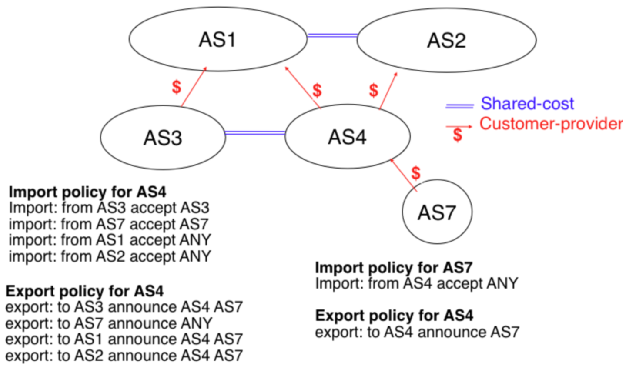
\includegraphics[width=11cm]{policies.png}
    \caption{Import export policies example}
\end{figure}

\subsubsection{The Border Gateway Protocol (BGP)}

Dans BGP chaque domain est identifié par un unique \textit{Autonomous System} number (AS).

BGP n'envois pas sa routing table entière mais le fait de manière incrémentale, càd en
envoyant uniquement les routes qui ont changé.

De plus BGP utilise TCP pour garantir le bon délivrement des BGP messages.

\paragraph{BGP session}

\paragraph{Etablisment} doit être fait manuellement pour des raisons de sécurité.

\paragraph{Messages}

\begin{enumerate}
    \item \textit{OPEN} : Quand la connection est établie, ça initialise la session et
        négocie d'option
    \item \textit{NOTifICATION} : Pour cloturer la session
    \item \textit{UPDATE} : Averti du changement d'une route. C'est le message le plus important et pour que le protocol soit efficace, le message doit minimiser le nombre de bit envoyé.
    \item \textit{KEEP ALIVE} : Averti que rien n'a changé (pour être sur que le router
        est toujours en vie)
\end{enumerate}

\paragraph{BGP update} = \{IP prefixe retié\}, \{IP préfixe ajouté\}, \{AS-Path\}

\subparagraph{ } Une route qui est envoyé doit d'abord passer l'\textit{export filter},
de même qu'une route reçue doit passer l'\textit{import filter}. Un BGP routeur est composée de 4 structures de donnée: 
\begin{itemize}
	\item Adj-RIB-In : Les routes que l'ont a apprises au routeur mais qui n'ont pas encore était filtré.
	\item Local-Routing-Information Base: Routes apprises après import filter.
	\item Fowarding Information Base: Mapping entre destination et meilleur route.
	\item Adj-RIB-Ouut : Route que le routeur apprend au voisin après application du export filter.

\end{itemize}
\paragraph{The BGP decision process}
En plus des import/export filter, il y a un algorithme qui choisit la meilleur route.
Ce choix est fait sur base des BGP attribut attaché à chaque route.

\paragraph{Local-pref}
Le premier attribut de cet algorithme est la local-preference, celui ci est attribué
selon l'import filter. (Highest value est préféré)

\subparagraph{Cheap link} On peut implémenté la préférence d'un lien peut couteux
plutôt qu'un autre via le local-pref en définissant les valeurs dans l'import filter.


\paragraph{Local-pref with customer->provider and shared cost}
\begin{enumerate}
    \item High local-pref pour les routes apprisent par le customer (\textit{provider->customer})
    \item Medium local-pref pour les shared-cose
    \item Low local-pref pour les routes apprisent par le provider (\textit{customer->provider})
\end{enumerate}


\paragraph{BGP convergence}
Certaines routing policies peuvent interférer entre elles et aboutir (en théorie),
à des ping-pong infini.

\paragraph{ } La convergence des BGP n'esy pas toujours garanti et verifier la
convergence global est un problème NP-complet.

\paragraph{Guideline to guarantee BGP convergence}
\begin{enumerate}
    \item Le graph est \textit{customer->provider} est acyclique
    \item AS préfére une route reçue d'un customer plutôt qu'une shared-cost
\end{enumerate}

\subsubsection{Structure global internet}
Les domains peuvent être divisé en 4 catégories par rapport à leurs role et leur position dans la topologie AS:
\begin{itemize}
	\item Tier-1 : Le noyau de l'Internet, ce sont les domaines qui n'ont pas de provider.
	\item Tier-2: Customer de Tier-1, ils ont des customers plus petit et partage les coût avec d'autre T2
	\item Tier-3 : Customer de Tier-1 et Tier-2 (stub domain ou petit ISP)
	\item Large content provider: Large datacenter, ils produisent une grandes parties des données échangées sur l'internet globale. Customer de T1 ou T2 mais souvent ils sont en shared-cost avec les T1 ou T2 (via IXP)

\end{itemize}

\subsection{Datalink layer technologie}

\subsubsection{The point to point protocol}
On se limite aux protocoles qui sont souvnet utilisés pour le \textbf{transport de paquets IP} entre hôtes et routeurs connectés par un lien point-to-point.

\paragraph{\textbf{Serial Line IP} (SLIP)} : C' est une technique de character 
stuffing appliqué aux paquets IP utilisant deux caractères spéciaux :
\begin{itemize}
    \item[-] \textsc{END} : en début et fin de paquet
    \item[-] \textsc{ESC} : devant un END s'il est dans les informations à transmettre
\end{itemize}

\begin{tabular}{cm{11cm}}
    \underline{Limitations} de SLIP :
    &
    \begin{itemize}
     \item Supporte uniquement la transmission de paquets IP
     \item Configuration manuelle des adresses IP entre host et routeur.
    \end{itemize}
\end{tabular}

\subparagraph{Note:} SLIP était surtout utilisé sur des liens $\leq 20Kps$ sur lequel
    des techniques de \textbf{compressions} des headers TCP/IP étaient indispensable.
    (\textit{Les header prenaient déja bcp de temps})

    $\to$ On exploitait la redondance de segment consécutif pour compresser

\paragraph{\textbf{Point-to-Point protocol} (PPP)} : Supporte IP et d'autres protocoles de la couche réseaux sur différents types de lignes de transmission. Il utilise le bit stuffing ou le character stuffing selon l'environnement où le protocole est utilisé.

PPP est une famille de 3 protocoles qui s'utilisent ensemble :
\begin{enumerate}
    \item Le \textit{Point-to-Point Protocol} : Technique de framing pour transporter les paquets dans la couche réseau.
    \item Le \textit{Link Control Protocol} : Utilisé pour négocier les options et authentifier la session (\textit{username/password, \ldots})
    \item Le \textit{Network Control Protocol} : Spécifique à chaque protocole de la couche réseau, il permet de négocier les options spécifiques au protocole. (\textit{IPv4's NCP négocie
        l'adresse IPv4})
\end{enumerate}

\subparagraph{Frame} :
Les champs Address (8) et Control (8) sont présentes pour des raisons de compatibilité. Le champ Protocol (16 bits) contient l'ID du type de protocole utilisé pour le transport de la trame PPP. 

PPP supporte des paquets de taille variable mais LCP peut négocier une taille de paquet maximum.
	
\begin{figure}[!ht]
    \centering
    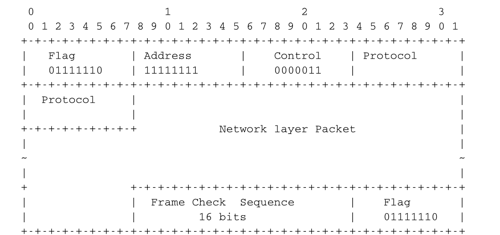
\includegraphics[width=10cm]{ppp_frame_format.png}
    \caption{Format d'une trame PPP}
\end{figure}
	
\begin{center}
\textit{PPP a fournit un accès dial-up (ligne commuté) aux fournisseurs d'accès Internet (ISP).
    Cet accès à internet se faisait via l'Extensible Authentification Protocol (EAP) par 
    mot de passe.
    Avec l'arrive de l'Asymmetric Digital Subscriber Lines (ADSL) et voulant réutiliser
    leur système d'authentification/facturation, IETF a dévellopé des spécifications
pour transporter des framesPPP sur d'autre réseaux que les point-to-point.}
\end{center}
	
\subsubsection{Ethernet}

\paragraph{Ethernet standard 1980} : 
\begin{itemize}
    \item \textbf{Vitesse}   : 10 Mbps  (\textit{3Mbps en 1970})
    \item \textbf{Slot time} : 51.2ms (\textit{minimun frame size = 64bytes})
        \begin{itemize}
            \item[$\to$] Equivaut à deux fois le temps que prend un impulsion électronique
                pour parcourir une longeur maximun entre deux noeuds.

                Attendre ce slot time permet de détecter les collisions en CSMA/CD
        \end{itemize}
    \item \textbf{Frame format} : 
        \begin{itemize}
            \item \textbf{Dest adresse} (48 bits) : multicast, broadcast et unicast.
                
                Il est placé en début de frame pour que le recepteur sache rapidement si
                elle lui est destiné ou non
            \item \textbf{Source adresse} (48 bits) : Uniquement unicast
            \item \textbf{Type} (16) : type du paquet transporté sur la couche réseau , \textbf{CRC} (32)
            \item 46bytes $<$ \textbf{Payload} $<$ 1500 bytes
        \end{itemize}

        Note que le début d'une frame Ethernet commence par un préambule
        utilisé par la pysical layer pour synchroniser les horloges.
    \item \textbf{Adresses} :
        \begin{itemize}
            \item Addresse global \textbf{unique} (MAC adresse) sur 48bits (\textit{permet d'allouer des
                gros blocs d'adresse au fabriquant})
            \item Définition d'adresse broadcast and multicast 
        \end{itemize}
\end{itemize}

\begin{figure}[!ht]
  \centering
  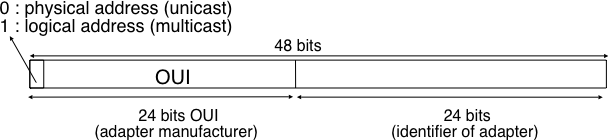
\includegraphics[width=9cm]{ethernet_address_format.png}
  \caption{MAC adresse format}
\end{figure}

\paragraph{ }Un réseau Ethernet fournit un \textbf{unreliable connectionless service}
(\textit{Avec unicast, multicast et broadcast}) tel que :
\begin{itemize}
    \item Very high probability of successful delivery ($\to$ utilisation de CSMA/CD)
    \item Transmission frame dans l'ordre ($\to$ topologie réseau ethernet = shared bus)
\end{itemize}
 
\begin{figure}[!ht]
    \centering
    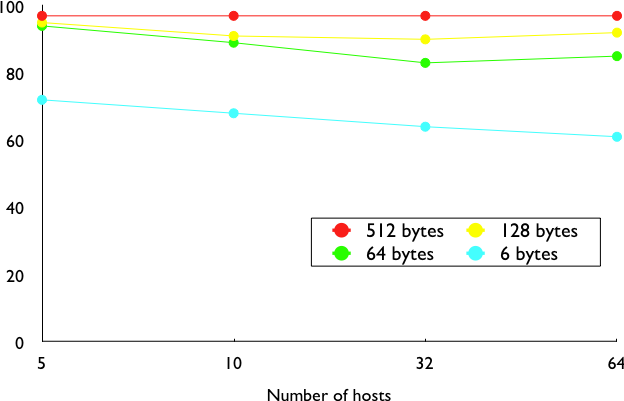
\includegraphics[width=6cm]{impact_of_frame_length_in_ethernet.png}
    \caption{Pourcentage d'utilisation de la ligne en fonction de frame size}
\end{figure}
    
\begin{table}[ht]
    \centering
  \begin{tabular}{c|c|c|c|c|c}
  Nom & Vitesse & Longueur du cable & Type de câble & Répéteurs & Topologie réseau \\
  10Base5 & 10 Mbps & 500 mètres & Cable coaxial & Oui & Shared bus\\
  10Base2 & & 185 mètres & Cable coaxial & Shared bus\\
  10BaseF & & & Lien optique & \\
  10BaseT & & & Câble torsadé & En étoile\\
  \end{tabular}
  \caption{Différentes couches physiques définie pour Ethernet}
\end{table}
      
      
\paragraph{Introduction paires torsadées} amène à deux changements majeurs sur Ethernet :
\begin{itemize}
    \item La topologie physique du réseau (Start shaped)
    \item L'obligation d'instaurer des hubs pour créer cette topologie 
\end{itemize}

\paragraph{Hub} : 

\begin{tabular}{m{10cm}m{5cm}}
    Un hub est un relais sur la couche physique qui
    \begin{itemize}
        \item reçoit un signal électrique sur une interfaces 
        \item le transmet sur toutes ses autres interfaces
        \item est capable de convertir des signaux électriques de deux
            couche physiques différentes (10BaseT$\to$10Base2)
    \end{itemize}
    &      
	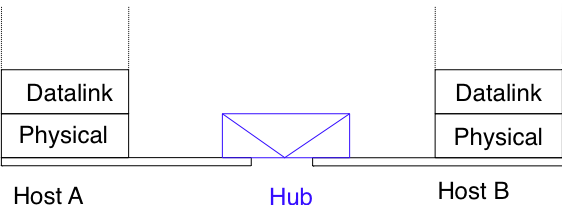
\includegraphics[width=5cm]{ethernet_hub.png}
\end{tabular}
      
Pour créer un réseau complexe avec des hubs, il faut faire attention à certains points :
\begin{enumerate}
    \item La topologie du réseau doit être un arbre     
    \item Il peut exister des collisions $\to$ CSMA/CD
    \item L'étendue du réseau est limitée par le slot time
\end{enumerate}
      
\begin{figure}[!ht]
    \begin{center}
    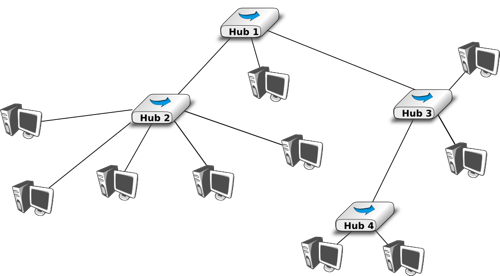
\includegraphics[scale=0.3]{hierarchical_ethernet_network.png}
    \caption{Un réseau Ethernet hiérarchique composé de hubs}
    \end{center}
\end{figure}

\paragraph{Le Fast Ethernet} est une technologie LAN qui permet d'aller jusqu'à 100Mbps en utilisant la fibre optique. Deux contraintes :
\begin{itemize}
    \item Supporter les paires torsadées (\textit{en couche physique on aurait préféré les câbles coaxiaux mais c'est chiant pour la maintenance})
    \item Utiliser le même format de frame qu'en 10Mbps (parce qu'à la base, ce lien de 100Mbps servait de lien entre 2 liens 10 Mbps). 
        
        $\to$ Pour préserver CSMA/CD : slot time = 5.12 microsecondes.
\end{itemize}
      
\paragraph{\textbf{Ethernet switches}}
Une autre solution pour améliorer les performances des LAN ethernets (\textit{que le fast ethernet}), est de rendre les hubs intelligents.

\paragraph{Switch} \textit{hubs intelligents} capable d'agir sur la couche datalink
et analyser l'adresse de destination de chaque frame et forwarder dans la direction
de la destination.

\begin{figure}[!ht]
    \centering
    \begin{tabular}{cc}
        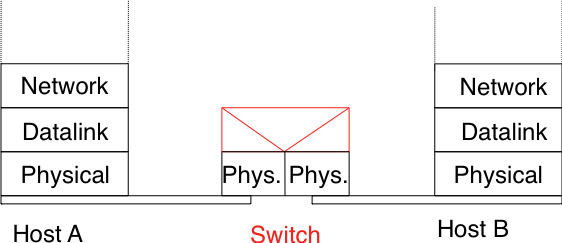
\includegraphics[width=6cm]{ethernet_switches.png} &
        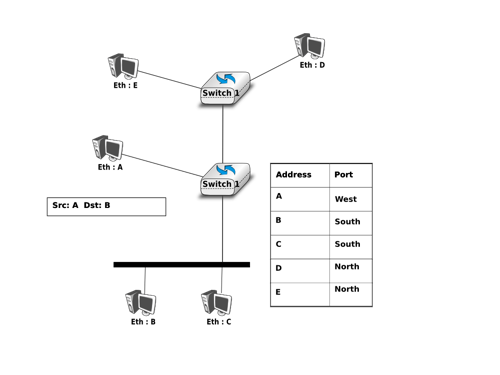
\includegraphics[width=6cm]{switch_mac_address_table.png}
    \end{tabular}
    \caption{Les switch Ethernet et table des adresses MAC}
\end{figure}
      
\subparagraph{Switch forwarding table} 
\begin{itemize}
    \item La table de forwarding fait le lien entre MAC adresse et port où forwarder

    \item Utilisations des MAC adresse (48 bits), un LAN ethernet est \textit{plug and play}.
        (\textit{On se connecte et on peut directement échanger})

        \begin{itemize}
            \item[$\to$] Nécessite une configuration automatique des tables des switchs
        \end{itemize}

    \item Avec les switchs, un host ne reçoit que les frames qui lui sont destinés 
        (\textit{unicast, multicast et broadcast}) ainsi que les frames dont le
        switch ne connait pas la destination

    \item[$\color{red}\bullet$]  \textcolor{red}{Attaque par dénide service}
        Taille des tables MAC est limité, un host peut envoyer plein de frame avec
        des adresses sources aléatoire et overflow le switch.
        \begin{itemize}
            \item [$\to$] Le switch devra broadcast toutes les frames reçue, et l'attaquant
                recevra donc tout les frames..
        \end{itemize}
\end{itemize}


Si  on  combine le  \textbf{MAC  address  learning} et  l'algorithme  de
forwarding,  on  peut gérer les réseaux en arbre qui n'ont pas de boucle
(pas de TTL, ni HopLimit)

(\textit{Cependant, un arbre est dangereux :  en cas de problèmes avec un lien le
réseau est scindé en deux.})

      
\paragraph{Spanning Tree Protocol} 
Permet de réduire un réseau à un \textbf{Spanning Tree}.
\begin{itemize}
    \item Les switches échangent les BPDU pour créer le spanning,
        Les BPDU sont envoyé avec \textsc{ALL\_BRIDGES} comme destination multicast
    \item Le plus petit 64bits identifier (48 lower avec MAC adresse, 16 higher
        permette à l'admin d'influencer le réseau) est élu \textbf{root}, et les branches
        sont composés avec les chemins les plus court permettant à tout les 
        switchs du réseau d'être atteint
\end{itemize}

\subparagraph{BPU} (:= <R, c, T, P>) contient :

\begin{itemize}
    \item L'identifiant du switch racine (R)
    \item Le coût du chemin le plus court entre le switch qui a envoyé le BPDU et la racine (c)
    \item L'identifiant du switch qui a envoyé le BPDU (T)
    \item Le numéro du port du switch qui a envoyé le BPDU (p)
\end{itemize}

\subparagraph{Priority vector} $V[q] = < T, c + cost(q), T, p, q>$

\subparagraph{Port} 
Chaque port d'un switch est \textbf{root, désigné} ou \textbf{bloqué}.
Un port est \textbf{root} est celui qui est le plus proche du switch racine!

\begin{table}[ht]
    \begin{center}
    \begin{tabular}{|c|c|c|c|}
        \hline
        Etat du port & Réception de BPDU & Envoi de BPDU & Gestion de trames de données \\
        \hline
        Bloqué & OUI & NON & NON \\
        Racine & OUI & NON & OUI \\
        Désigné & OUI & OUI & OUI \\
        \hline
    \end{tabular}
    \end{center}
    \caption{Transmission des BPDU selon l'état de chaque port}
\end{table}

\subparagraph{Fonctionnement} 

\begin{itemize}
    \item Chaque switch ecoute les BPDU sur ses ports
    \item Pour les BPDU reçu, il calcule le \textbf{priority vector} associé au port d'où vient le BPDU et stocké le \textbf{meilleur pour chaque port}
    \item Switch root est connu en regardant le plus petit identifiant stocké dans la
        table des priority vector
        \begin{enumerate}
            \item Le switch root à $<R,O,R,p>$
            \item Les autres switch au $<R, c, S, p>$ connaissent leur root port (celui avec le meilleur
                priority vector)
        \end{enumerate}
    \item Un port est designé si le BPDU du switch est meilleur que le priority vector
        du port sinon il est bloqué.
    \item[$\to$] R : root switch, S : identifiant switch, c : cost best priority vector, p : number port d'où vient le BPDU
\end{itemize}

\subparagraph{Quand la version est stable}
Le switch racine envoie régulièrement son propre BPDU qui est reçu sur le port Root des switchs directement connectés à la racine.

\begin{itemize}
    \item Les switches écoutent tout de même sur le port Bloqué, mais si la topologie du réseau est stable, normalement aucun BPDU ne doit arriver dessus.
    \item Lors du calcul du Spanning Tree, \textbf{aucune donnée} n'est transmise dans le réseau.
        
        Après le spanning tree, l'algorithme de MAC learning se lance.
\end{itemize}


\subparagraph{Recover failure}
Les switches, ports et liens peuvent foirer dans un réseau Ethernet avec des switches : quand ça arrive, il faut refaire le spanning tree. Pour les détecter, on envoie des BPDU régulièrement (le BPDU contient deux autres champs : son âge et l'age maximum).
\begin{itemize}
    \item Age=0 pour le root et il est incrémenté de 1 dés qu'il passe par un switch
    \item Les switch stock age et l'incrémente chaque seconde. Si il dépasse le
        max age, il y a donc une erreur et on refait STP
\end{itemize}

\paragraph{Les Virtual LANs} sont un ensemble de ports dans un ou plusieurs switches. Un switch peut gérer plusieurs LANs séparément et applique l'algorithme de MAC learning sur chacun des VLANs sans partager leurs informations respectives.

\begin{figure}[ht]
    \begin{center}
      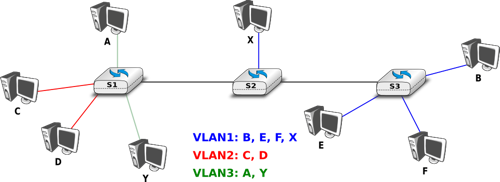
\includegraphics[width=9cm]{virtual_local_area_networks.png}
      \caption{Trois Virtual Area Networks connectés par des switches}
    \end{center}
\end{figure}


Pour permettre au switch de distinguer les VLAN on met un identifiant à chaque VLAN qu'on met dans chaque header de frame échangée. Ce header est inséré directement après l'adresse MAC dans la frame Ethernet (avant EtherType).
\begin{figure}[!ht]
    \begin{center}
    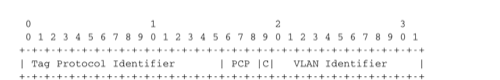
\includegraphics[width=14cm]{header_vlan.png}
    \caption{Header VLAN (802.1q)}
    \end{center}
\end{figure}

\begin{itemize}
    \item Le Tag Protocol mis à 0x8100 permet au receveur de détecter la présence de ce header.
    \item Le Priority Code Point (PCP) permet de définir des priorités dans les trames. 
    \item Le champ C permet la compatibilité entre Ethernet et les réseaux Token Ring. 
    \item Le dernier champ est l'identifiant de la VLAN (0 = pas un VLAN; 4095 est réservé).
\end{itemize}

\subsubsection{802.11 Wireless networks}

Le spectre radio est une ressource limitée partagée entre tous.
Il est reglementé par les instituions internationales et les gouvernements pour éviter les interférences. La seule exception de non-règlementation sont les ondes ISM (Industrial, Scientific and Medical). On utilise la bande 2400-2500Ghz pour le WiFi comme pour les micro-ondes, le bluetooth,... (il peut donc y avoir des interférences).

\paragraph{Standard 802.11}
IEEE a créé ce standard pour les familles de réseaux sans fil WIFI:

\begin{center}
\begin{tabular}{|c|c|c|c|c|}
\hline
Standard & Fréquence & Débit typique & Bande passante max & Portée (m) intérieur/extérieur \\
\hline
802.11 & 2.4 Ghz & 0.9 Mbps & 2 Mbps & 20/100 \\
802.11a & 5 Ghz & 23 Mbps & 54 Mbps & 35/120 \\
802.11b & 2.4 Ghz & 4.3 Mbps & 11 Mbps & 38/140 \\
802.11g & 2.4 Ghz & 19 Mbps & 54 Mbps & 38/140 \\
802.11n & 2.4-5 Ghz & 74 Mbps & 150 Mbps & 70/250 \\
\hline
\end{tabular}
\end{center}

Le wifi reprend CSMA/CA et la même architecture/frame que Ethernet.

L'architecture des réseaux WiFi est différente des LAN. Il y a deux types de réseaux WiFi : 
\begin{itemize}
    \item indépendant/adhoc : Quand on ne le relie pas à Internet (imprimante wifi) 
    \item infrastructure : contiennent un ou plusieurs points d'accès attachés à un LAN (souvent Ethernet) qui lui est connecté à Internet.
\end{itemize}

Le payload maximum théorique en 802.11 est de 2324 bytes mais le standard le limite à 1500.

\begin{figure}[!ht]
    \centering
    \begin{tabular}{cc}
        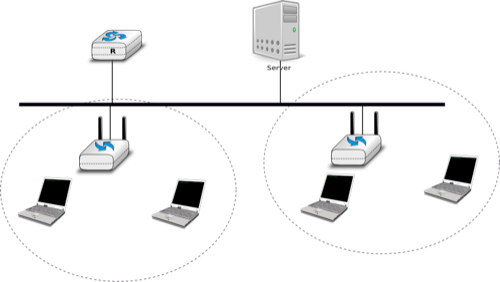
\includegraphics[width =6cm]{wifi_infrastructure.png} &
         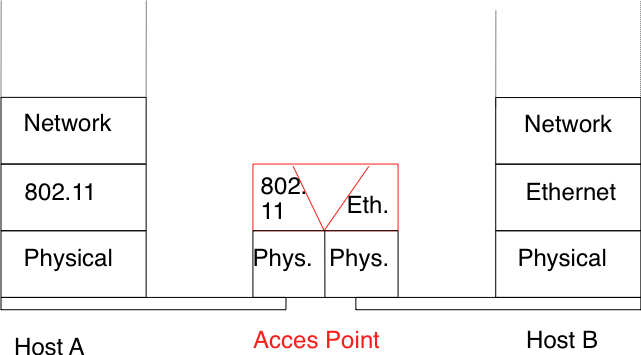
\includegraphics[width=6cm]{wifi_access_point.png}\\
         Réseau infrastructure 802.11 & Point d'accès WiFi
     \end{tabular}
\end{figure}

\begin{figure}[!ht]
    \centering
    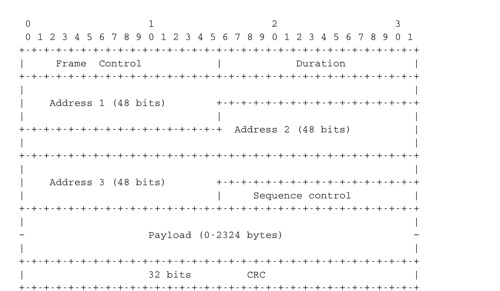
\includegraphics[width=12cm]{wifi_data_frame_format.png}
    \caption{Format des trames de données en 802.11}
\end{figure}

Format des frames en 802.11 :
\begin{itemize}
    \item Frame Control : indique le type de trame (data, RTS/CTS/ ack, management frames,...), si la trame est envoyée depuis un LAN,... 
    \item Duration : permet de réserver un temps de transmission (temps de transmission de l'ack + SIFS pour les data ; 0 pour multi/broadcast). 
    \item Sequence Control : contient un numéro de séquence incrémenté pour chaque trame de données.
    \end{itemize}

On se rend compte qu'il y a 3 champs d'adresse :
\begin{enumerate}
    \item L'adresse MAC du point d'accès
    \item L'adresse MAC de la source WiFi 
    \item L'adresse de destination final sur le LAN.
\end{enumerate}

\paragraph{Unreliable connectionless service}
Malgré l'utilisation d'acquittements, la couche 802.11 ne fournit qu'un service unreliable connectionless comme Ethernet. Les acquittements sont utilisés pour minimiser la probabilité de duplication de trame, ils n'assurent pas la livraison des données (haute probabilité mais pas garantie).

\paragraph{Encapsulation}
L'encapsulation d'IP sur 802.11 ajoute 6 bytes au header 802.11, 4 bytes pour LLC/SNAP et 2 bytes de Ethernet Type (IP ou ARP).

\begin{figure}[!ht]
\begin{center}
    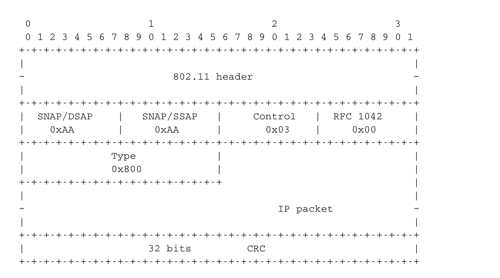
\includegraphics[width=12cm]{ip_over_wifi.png}
  \caption{Paquet IP encapsulé dans une trame WiFi 802.11}
\end{center}
\end{figure}

\section{Algorithmes}
   \subsection{MAC Address Learning par les switches}
	  \lstset{keepspaces=true, keywordstyle=\color{red!70}, commentstyle=\color{blue!60}}
	  \begin{center}
	  \framebox{\begin{minipage}{0.9\linewidth}
	     \lstinputlisting[language=Python]{mac_address_learning.py}
	  \end{minipage}}
	  \end{center}

\biblio

\end{document}
